\documentclass[letterpaper,12pt]{article}

% Import packages from .sty file.
\usepackage{imports}


% Set up the title.
\title{From Value Added to Welfare Added: A Social Planner Approach to Education Policy and Statistics.}
\author{Tanner S Eastmond\thanks{Department of Economics, University of California, San Diego} \and Nathan Mather\thanks{Department of Economics University of Michigan} \and Michael Ricks$^\dagger$ \and Julian Betts$^*$}
\date{\vspace{-8ex}}




%%%%%%%%%%%%%%%%%%%%%%%%%%%%%%%%%%%%%%%%%%%%%%%%%%%%%%%%%%%%%%%%%%
%%%%%%%%%%%%%%%%%%%%%%%%%%%%%%%%%%%%%%%%%%%%%%%%%%%%%%%%%%%%%%%%%%

\begin{document}
\maketitle




%%%%%%%%%%%%%%%%%%%%%%%%%%%%%%%%%%%%%%%%%%%%%%%%%%%%%%%%%%%%%%%%%%
%%%%%%%%%%%%%%%%%%%%%%%%%%%%%%%%%%%%%%%%%%%%%%%%%%%%%%%%%%%%%%%%%%
%%%%%%%%%%%%%%%%%%%%%%%%%%%%%%%%%%%%%%%%%%%%%%%%%%%%%%%%%%%%%%%%%%

\begin{abstract}
    A major goal of Value Added Measures (VAM) is to evaluate and compare teachers. These measures both perform relatively well in identifying better teachers and capture relevant information about the long-term effects teachers have on students. Despite this and the increasing reliance on standard mean VAM to measure teacher performance, there seems to be a philosophical disconnect between this and education policy with distributional goals, such as No Child Left Behind. We propose a simple welfare framework allowing policymakers to differentially weight students and a set of more flexible VAM to capture heterogeneity in teacher value added. We show that our flexible VAM perform well in simulations then show in data from San Diego Unified School District (SDUSD) that there is appreciable heterogeneity in teacher value added and that this heterogeneity translates to real-world outcomes for students. Lastly we show that, despite the allure as seemingly `utilitarian' estimates, using standard mean VAM to evaluate teachers implies an undesirable set of student weights and suggest low cost policies to improve student outcomes without infusing more resources into the schools.
\end{abstract}




%%%%%%%%%%%%%%%%%%%%%%%%%%%%%%%%%%%%%%%%%%%%%%%%%%%%%%%%%%%%%%%%%%
%%%%%%%%%%%%%%%%%%%%%%%%%%%%%%%%%%%%%%%%%%%%%%%%%%%%%%%%%%%%%%%%%%
%%%%%%%%%%%%%%%%%%%%%%%%%%%%%%%%%%%%%%%%%%%%%%%%%%%%%%%%%%%%%%%%%%

\section{Introduction}

Over the past two decades teacher value added measures (VAM) have become increasingly common methods for evaluations of relative teacher performance. These measures are motivated by the fact that comparing teachers based on average student achievement in their classes would result in unfair assessments of teachers who are assigned to teach lower achieving classes, and whose students---often through little or no fault of their own--tend to have lower test scores. Intuitively value added measures compare teachers not on the level of student achievement in their class, but on the gains their students experience (thus the value ``added'').

While test score gains are certainly not the only mark of an effective teacher, research has demonstrated that teachers with high value added scores have long-term impacts on their students' graduation rates and earnings \citep{chetty2014measuring2}. Furthermore, research has shown that teachers with high test-score value added tend to have higher value added on student attendance and on reducing student suspensions and retention \citep{pope2017multidimensional}.\footnote{This positive association is not perfect and there are many teachers with high non-testing value added who have lower test-score value added.} 

Standard value added measures focus on the average impact on students in a teacher's class; however, research has also made it clear that not all students experience the same gains under the same teacher. For example, the ``teacher-match effect'' reveals that students who are assigned effective same-gender or same-race teachers experience greater test score gains in the present and future than those who do not \citep{dee2005teacher,delhommer2019highschool}. Furthermore, teachers on the ground in classrooms suggest that teaching higher- or lower-achieving students often requires that they utilize and employ very different skills to keep students engaged and energized about learning. These types of differences are lost to value added measures because they average across all of a teacher's students in a given year. Throughout our paper we also refer to heterogeneity in teacher value added across the student achievement distribution as variation in teacher `match quality' for brevity.

We first attempt to examine teacher match quality in a set of econometric simulations where we compare standard value added estimators to several more flexible value added estimators that allow for differences in teacher match quality. The estimators we explore in these simulations allowing for flexibility in teacher value added along the achievement distribution are a simple standard value added estimator including interacted bins for prior achievement, kernel regression, and quantile regression. These simulations explore the feasibility and reliability of the estimators under various empirical circumstances and compare this to standard value added estimates. The main takeaways from our simulations are that under a variety of student assignment policies and welfare objectives our more flexible value added estimators recover the true ranking of teachers as well as or better than standard value added.

We then take these estimators to linked student-teacher data from San Diego Unified School District (SDUSD) spanning the 2001-2002 through 2012-2013 school years. We find evidence of differential effectiveness along the achievement distribution both within and across teachers. In particular, we find evidence that value added is different for above and below median students in 96\% of teachers with English language (ELA) and 97\% with mathematics. Furthermore, we show that this heterogeneity matters for long-term student outcomes. A below median student in a class where the teacher has 1 standard deviation higher value added in ELA for below median students is 1 percentage points more likely to enroll in a 2 year college. However, teachers with high below median value added for do not move the needle on outcomes such as enrolling in a 4 year college or graduating with a Bachelor's degree within 6 years of high school. Teachers with higher above median value added drive these latter outcomes. An above median student is 3.1 pp more likely to enroll in a 4 year college and 2.6 pp more likely to earn a Bachelor's degree for each standard deviation higher above median math value added (the numbers are 4.5 and 3.3 for ELA).

With this estimated heterogeneity in hand, we turn to the educational policy that often has goals for specific student sub-populations. Standard mean VAM seem to have the intuitive appeal of treating students equally (a `utilitarian' weighting). However, we show that these measures induce an unintuitive weighting over students that is actually regressive. This is at odds with the goals of most education policy, which tends to focus on underrepresented or struggling students. With our welfare framework we allow the policymaker to explicitly choose the weighting over students, which allows us to correctly identify which teachers are moving forward the policy agenda and goals. This can then translate into various actionable conclusions, including, among other things, teacher/student reassignment across classrooms, incentive schemes, or identifying teachers for training purposes.

Our work in this study fits closely with several previous papers. First, \citet{lockwood2009} explore whether the effect of teachers on students is heterogeneous along the achievement distribution. They find significant, though modest heterogeneity in teachers' effects on students with different prior achievement. The author's results are, however, quite sensitive to the specification. The second paper that fits closely with our current work is \citet{condie2014teacher}. The authors in this study examine the assumption for value added estimates that effects are homogeneous across different students. Their results suggest that this assumption is likely to be wrong, and they show in various simulations that assigning teachers to students they are comparatively better at teaching could improve student test scores.

We contribute to these studies and the other literature in several ways. First, we provide a practical option for estimating heterogeneity in teacher effects and describe under what conditions they work well relative to standard value added estimates. Second, we show that these measures are strong predictors for real-world outcomes, and that teachers with different value added along the achievement distribution differentially impact these real-world outcomes. Last, we show that standard mean VAM induce an unexpected welfare weighting across students and allow policy makers to make the weighting explicit in order to improve the ranking of teachers under any given policy agenda and goals.

Our paper continues in Section \ref{sec: Data} by discussing the SDUSD and the data. We then build our welfare framework for VAM in Section \ref{sec: Welfare} and discuss our estimates for standard value added and our more simple flexible value added in Section \ref{sec: Estimation} In that section we also discuss our simulations and real-world results for our various estimates. This is followed by a discussion of the welfare weighting induced by standard mean VAM and policy applications in Section \ref{sec: Regressive VA}. We end with robustness checks in Section \ref{sec: Robust}, after which we conclude.




%%%%%%%%%%%%%%%%%%%%%%%%%%%%%%%%%%%%%%%%%%%%%%%%%%%%%%%%%%%%%%%%%%
%%%%%%%%%%%%%%%%%%%%%%%%%%%%%%%%%%%%%%%%%%%%%%%%%%%%%%%%%%%%%%%%%%
\section{Background and Data}\label{sec: Data}

The primary data for our project are teacher-student linked data from the San Diego Unified School District (SDUSD) covering the 2001-2002 through 2017-2018 school years. These data include around 424,926 unique students and 7,509 unique teachers across 153 schools. These data include rich information on student outcomes including test scores, attendance, and high school performance. They also include teacher characteristics such as gender, age, teaching credentials, and teaching experience.

Before fall 2013, students in grades 2-11 were required to take the California Standards Tests (CST), which a series of tests intended to reflect the state's curriculum in each subject. In our analysis we focus on elementary students taking the CST in English and mathematics for whom we have at least two years of test data, or those in grades 3-5 between 2001 and 2013, for whom we can identify a unique teacher. After fall 2013 these tests were replaced with the California Assessment of Student Performance and Progress (CAASPP) Program, so to avoid issues with comparing across testing regimes we focus on the earlier period. This leaves us with an analysis sample of 150,406 unique students, 5,416 unique teachers, and 360,619 student-year observations. On average we observe students in our sample for 3 years and teachers for 7 years. We assume that all students assigned to the same teacher in a year are in the same class, and this implies that classes in our sample had 25 students on average. Based on the simulations that we run, we also require that teachers included in our analysis taught a minimum of 50 students with consecutive years of test scores, leaving 2,165 teachers for our analysis.

Additionally, we use the National Student Clearinghouse Data for information on long-term student outcomes. These data include information on post-secondary outcomes for the students in our sample. Specifically they include whether a student attended a 2 or 4 year university in the 4 years following high school graduation, how many years were attended in that span, what degree, if any, was earned, and what the field of study was.

Table \ref{tab: summary} gives some descriptive statistics for our sample.

\begin{table}[ht]
    \centering
    \caption{Descriptive Statistics for Sample}
    \input{"tables/Sample Description"}
    \label{tab: summary}
    \caption*{\scriptsize \textit{Notes:} Standard deviations in parentheses. Test scores are standardized based on the overall mean and standard deviation for California. Outcomes with stars are not available for all students in the indicated sample. The `All Teachers' includes all teachers satisfying our sample requirements, `$\geq$ 50 Students' includes only teachers who have a minimum of 50 students with consecutive years of available test scores, and `$\geq$ 200 Students' is the same but with 200 students.}
\end{table}

\noindent SDUSD has a large fraction of Hispanic students, around 47 percent, many of whom were English learners at some point. Roughly a quarter of the remaining students are white, 13 percent are black, and 16 percent are Asian. Nearly 90 percent of students in the district graduate from high school, and around three quarters of students enroll in some college following high school.




%%%%%%%%%%%%%%%%%%%%%%%%%%%%%%%%%%%%%%%%%%%%%%%%%%%%%%%%%%%%%%%%%%
%%%%%%%%%%%%%%%%%%%%%%%%%%%%%%%%%%%%%%%%%%%%%%%%%%%%%%%%%%%%%%%%%%
%%%%%%%%%%%%%%%%%%%%%%%%%%%%%%%%%%%%%%%%%%%%%%%%%%%%%%%%%%%%%%%%%%
\section{A Simple Framework for ``Welfare Added''}\label{sec: Welfare}

Consider a scenario where we have $N$ students. Each student is assigned to a teacher each year, indicated by index $j(i,t)$. Each student has a current year test score $y_{it}$, past year test score $y_{i,t-1}$, and demographic characteristics $x_{it}$. Let $v(y_{it}, y_{i,t-1}, x_{it})$ be the value that student $i$ gains (e.g. actual achievement minus predicted achievement) and $\omega(y_{i,t-1}, x_{it})$ be the weight assigned to student $i$ by the social planner based on past test scores and current demographic characteristics. Then the ``welfare added'', $W_j$, of teacher $j$ is given by the following:

    \begin{equation}\label{eq: welfare}
        W_j = \sum_{i \in \{k : j(k, t) = j\} } \omega(y_{i,t-1}, x_{it})v(y_{it}, y_{i,t-1}, x_{it})
    \end{equation}
    
\noindent Thus each teacher improves social welfare by the amount of the weight assigned multiplied by the gain of each student taught by that teacher.

In this framework, a teacher's standard value added is the following (this is called the `Average Residual' approach to calculating standard value added and is algebraically the same as including teacher dummies in the full regression):
    
    \begin{equation*}
        W_j^{VA} = \sum_{i \in \{k : j(k, t) = j\} } \frac{y_{it} - \hat{y}_{it}}{N_j}
    \end{equation*}

\noindent where $N_j$ is the number of students taught by teacher $j$ and $\hat{y}_{it}$ is predicted achievement for student $i$. Since $\omega(y_{i,t-1}, x_{it}) = 1/N_j$ in this setting, standard value added estimates seem to weight all students equally, inducing a `utilitarian' weighting. We argue in Section \ref{sec: Regressive VA} that this is actually a mirage, and that because of estimation problems build into $\hat{y}_{it}$ the induced weighting for standard value added is not quite so simple.




%%%%%%%%%%%%%%%%%%%%%%%%%%%%%%%%%%%%%%%%%%%%%%%%%%%%%%%%%%%%%%%%%%
%%%%%%%%%%%%%%%%%%%%%%%%%%%%%%%%%%%%%%%%%%%%%%%%%%%%%%%%%%%%%%%%%%
%%%%%%%%%%%%%%%%%%%%%%%%%%%%%%%%%%%%%%%%%%%%%%%%%%%%%%%%%%%%%%%%%%
\section{Estimating Value Added}\label{sec: Estimation}

%%%%%%%%%%%%%%%%%%%%%%%%%%%%%%%%%%%%%%%%%%%%%%%%%%%%%%%%%%%%%%%%%%
%%%%%%%%%%%%%%%%%%%%%%%%%%%%%%%%%%%%%%%%%%%%%%%%%%%%%%%%%%%%%%%%%%
\subsection{Standard Mean Value Added Measures}

A rich literature exists on estimating mean VAM \citep[see, for example,][]{Koedel2015,chetty2014measuring1,guarino2015can,guarino2015evaluation, dieterle2015principals}. As explored in the deep literature, many modelling decisions must be made when estimating mean VAM. Key decisions include whether to model VAM as level test scores on lagged test scores (regress $y_{it}$ on $y_{i,t-1}$ or as a `gain-score' model ($\Delta y_{it} = y_{it} - y_{i,t-1}$ as the dependent variable); to include student fixed-effects or to rely on observables; to include school fixed-effects or to rely on observables; and to apply Bayesian shrinkage to the estimates or not.

One key simulation study, \cite{guarino2015can}, explored these issues. The authors compared the performance of various modelling choices under a gambit of student grouping and teacher assignment policies and find that the levels on lags model without student fixed-effects best recovered true teacher effectiveness.

Several other important studies explore further issues. One of these major issues is how biased mean VAM are. \cite{kane2013have} find that experimental and standard VAM estimates were quite close. These findings are corroborated by \cite{chetty2014measuring1}, who study bias in several ways. They omit details from students and families from IRS data and compare results with and without data on teachers who switched schools, concluding that biases in standard VAM are quite small as long as controls for past test scores are included. One counterpoint, \cite{rothstein2010teacher} shows that future teachers can predict current year learning, suggesting that standard VAM do not accurately reflect teacher effectiveness. However, this study has been raised into question by \cite{goldhaber2015assessing, koedel2011does}; and \cite{guarino2015can}.

Another key issues is what other covariates to include in addition to lagged test scores. \cite{chetty2014measuring1} in particular suggest that lagged test scores are by far the most crucial controls, and that omitting other controls led to negligible increases in bias. Including multiple years of consecutive test scores can further reduce bias, but this approach is costly since we lose additional years of data.

The last key issue we will highlight is that of Bayesian shrinkage. Though it is becoming more widespread \citep{Koedel2015}, \cite{guarino2015evaluation} find that Empirical Bayes models perform well unless students are not randomly assigned to teachers. However, they find that the standard VAM approach of regressing levels on lags performs best under a variety of scenarios.

We do our best to follow best practices from this literature. In particular, our estimating equation for the Standard value added is given by the following:

    \begin{equation}\label{eq: standard}
        y_{it} = \beta_1 y_{i,t-1} + \gamma_{j(i,t)} + \delta X_{it} + \varepsilon_{it}
    \end{equation}
    
\noindent where $y_{it}$ is current year test score in English language or Mathematics, $y_{i,t-1}$ is the lagged test score in the same subject, $\gamma_{j(i,t)}$ are teacher fixed-effects (which give our value added estimates), and $X_{it}$ is a vector of controls including lagged test score in the other subject, lagged classroom average test scores in both subjects, lagged school average test scores in both subjects, whether the student was ever an English learner, whether the student was ever in special education, student gender, student race, grade fixed-effects, and year fixed-effects. Standard errors are clustered at the school level.




%%%%%%%%%%%%%%%%%%%%%%%%%%%%%%%%%%%%%%%%%%%%%%%%%%%%%%%%%%%%%%%%%%
%%%%%%%%%%%%%%%%%%%%%%%%%%%%%%%%%%%%%%%%%%%%%%%%%%%%%%%%%%%%%%%%%%
\subsection{Two-Bin Value Added}

We start with the simple case of standard value added as given above, but we allow teachers to have differential effects for students above and below the median of prior achievement (as measured by past year test scores). Our specification for the above and below median bins estimate is the following:

    \begin{equation}\label{eq: bins}
        y_{it} = \beta_1 y_{i,t-1} + \beta_2 \mathbbm{1}\{y_{i,t-1} \in bin_{high}\}
        + \sum_{k=low, high}\sum_{i}\beta_k \gamma_{j(i,t)} \mathbbm{1}\{y_{i,t-1} \in bin_k\} + \delta X_{it} + \varepsilon_{it}
    \end{equation} 
    
\noindent where all is as in equation \ref{eq: standard} except now we include an indicator for whether student $i$ has a lagged test score above median that we also interact with the teacher fixed-effects. In particular, $\mathbbm{1}\{y_{i,t-1} \in bin_{high}\} = 1$ if $y_{i,t-1}$ is above the median of prior year test scores and $\mathbbm{1}\{y_{i,t-1} \in bin_{low}\} = 1$ if it is below the median.

We start here because it allows for heterogeneity in a transparent and intuitively appealing way. Additionally, some of the estimation problems we describe below become much more difficult as the number of bins increases.



%%%%%%%%%%%%%%%%%%%%%%%%%%%%%%%%%%%%%%%%%%%%%%%%%%%%%%%%%%%%%%%%%%
%%%%%%%%%%%%%%%%%%%%%%%%%%%%%%%%%%%%%%%%%%%%%%%%%%%%%%%%%%%%%%%%%%
\subsection{Econometric Simulations}

In these simulations we compare traditional value added estimates, as given by equation \ref{eq: standard}, with three different estimators that allow for heterogeneity in teacher value added along the student achievement distribution: traditional estimates including interacted indicator variables for prior achievement bins, kernel regression, and quantile regression.

We ask how well our alternative estimators perform relative to the traditional estimates under a variety of different assumptions and welfare policies. In particular, these assumptions include varying levels of match quality differences and overall ability differences between teachers, sorting of students into classrooms, and peer effects. The welfare policies we consider are where the policy maker targets all student improvement equally, targets students under a certain threshold, or targets students in a particular part of the distribution. For brevity we refer to these policy environments respectively `utilitarian', `rawlsian', and `selected group'. Our ultimate metric of success for various estimators is how well they uncover the `true' ranking of teachers. We define the `true' ranking of teachers to be the actual ranking of which teachers best push forward the given policy goals, or alternatively which teachers are most proficient at increasing welfare-weighted test scores. In particular we consider how well the estimators uncover the ranking in a Monte Carlo setting (if they are consistent for the truth).

We find that, regardless of the student assignment policy, the relative importance of overall ability and match quality matter greatly. If overall ability to teach all students swamps any match quality all estimators recover the true ranking of teachers equally well, but the standard value added estimates are much more precise. However, if match quality is relatively important then the standard value added estimates mis-rank teachers in predictable ways. In particular, they give more credit to teachers who teach the median students well rather than the target population of students (as a side note, if the target population for the policy maker is the median student, then standard value added measures perform quite well). We also derive the rule of thumb from these simulations of limiting our sample to teachers who have at least 50 students with consecutive test scores.


%%%%%%%%%%%%%%%%%%%%%%%%%%%%%%%%%%%%%%%%%%%%%%%%%%%%%%%%%%%%%%%%%%
%%%%%%%%%%%%%%%%%%%%%%%%%%%%%%%%%%%%%%%%%%%%%%%%%%%%%%%%%%%%%%%%%%
\subsection{Within Teacher Heterogeneity}

First, our work shows that there is significant heterogeneity across teachers in their overall value added as well as in their individual bin estimates. This is consistent with prior work and a broadly accepted fact, so we focus in this paper on within teacher differences in value added. We first perform a series of simple t-tests for the equality of the high bin estimate with the low bin estimate for each teacher. As shown in Figures \ref{fig: ELA ttest} and \ref{fig: math ttest}, we find statistical evidence of heterogeneity across bins for 96\% of teachers with their ELA value added and for 97\% of teachers with their math value added. 

\begin{figure}[ht]
    \centering
    \caption{Histogram of P-Values for T-Test of ELA Low Bin = High Bin}
    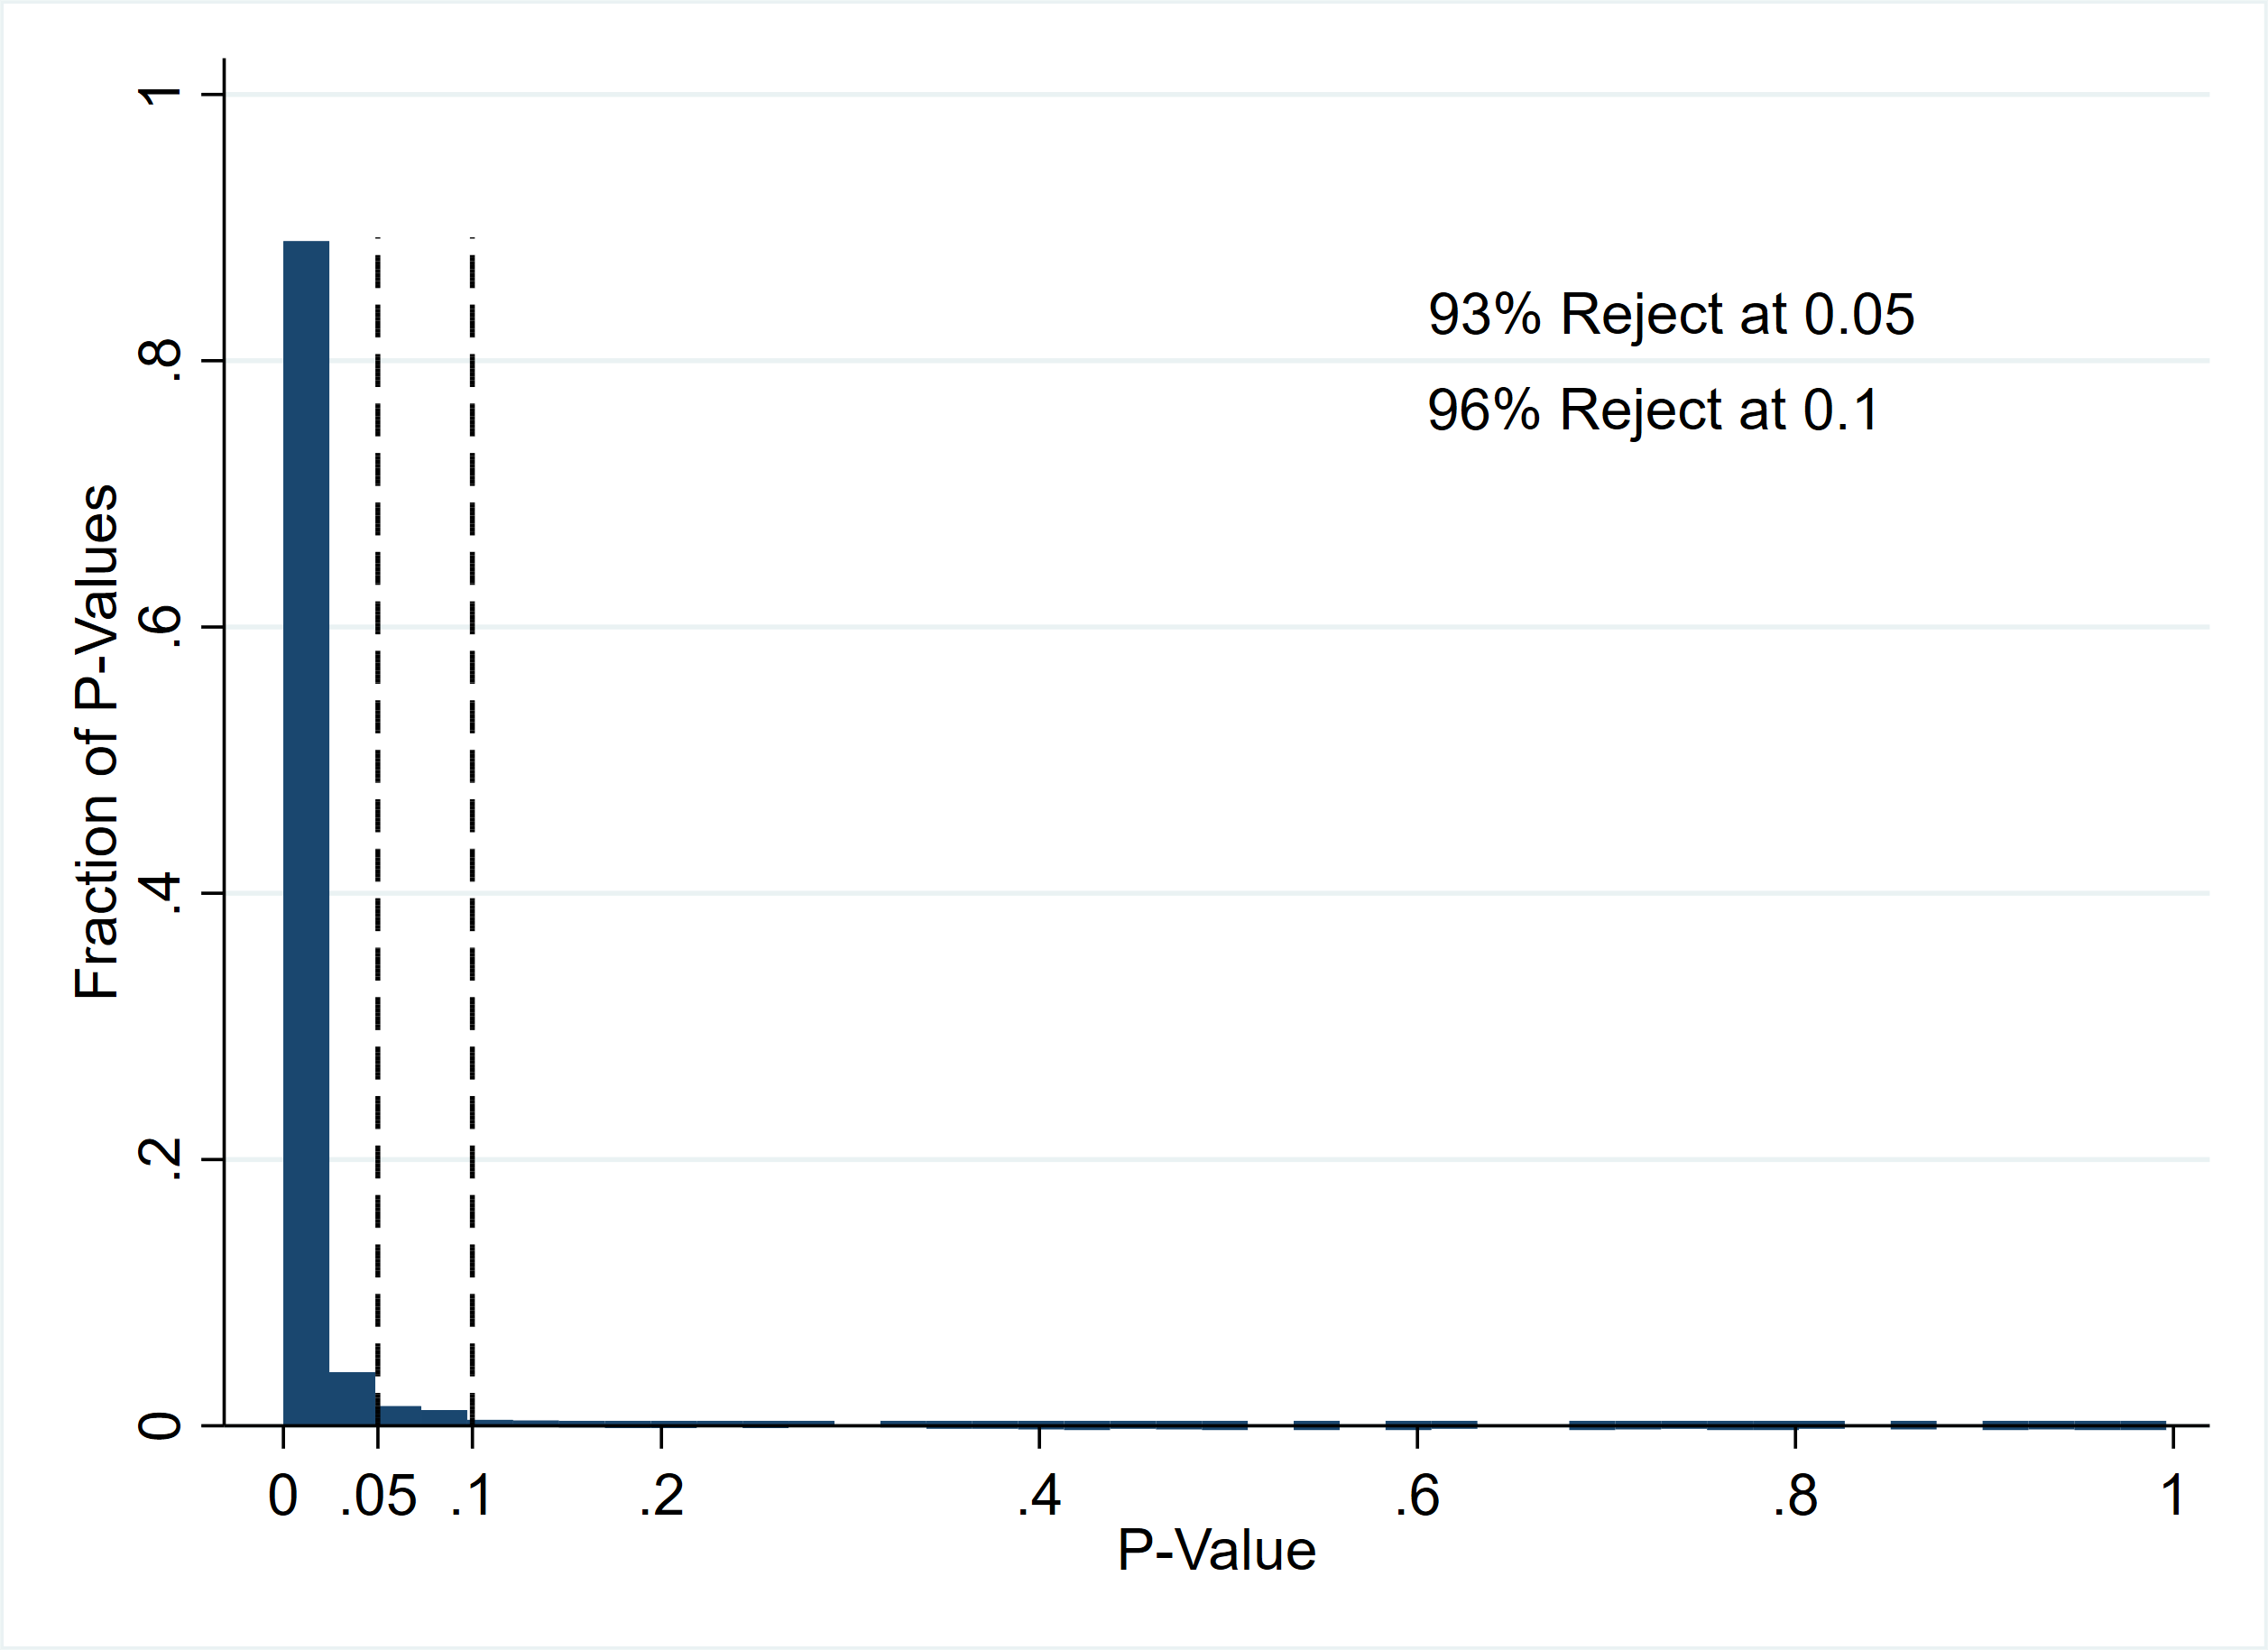
\includegraphics[width=\textwidth]{figures/ELA_T_Test_Hist.png}
    \label{fig: ELA ttest}
\end{figure}

\begin{figure}[ht]
    \centering
    \caption{Histogram of P-Values for T-Test of Math Low Bin = High Bin}
    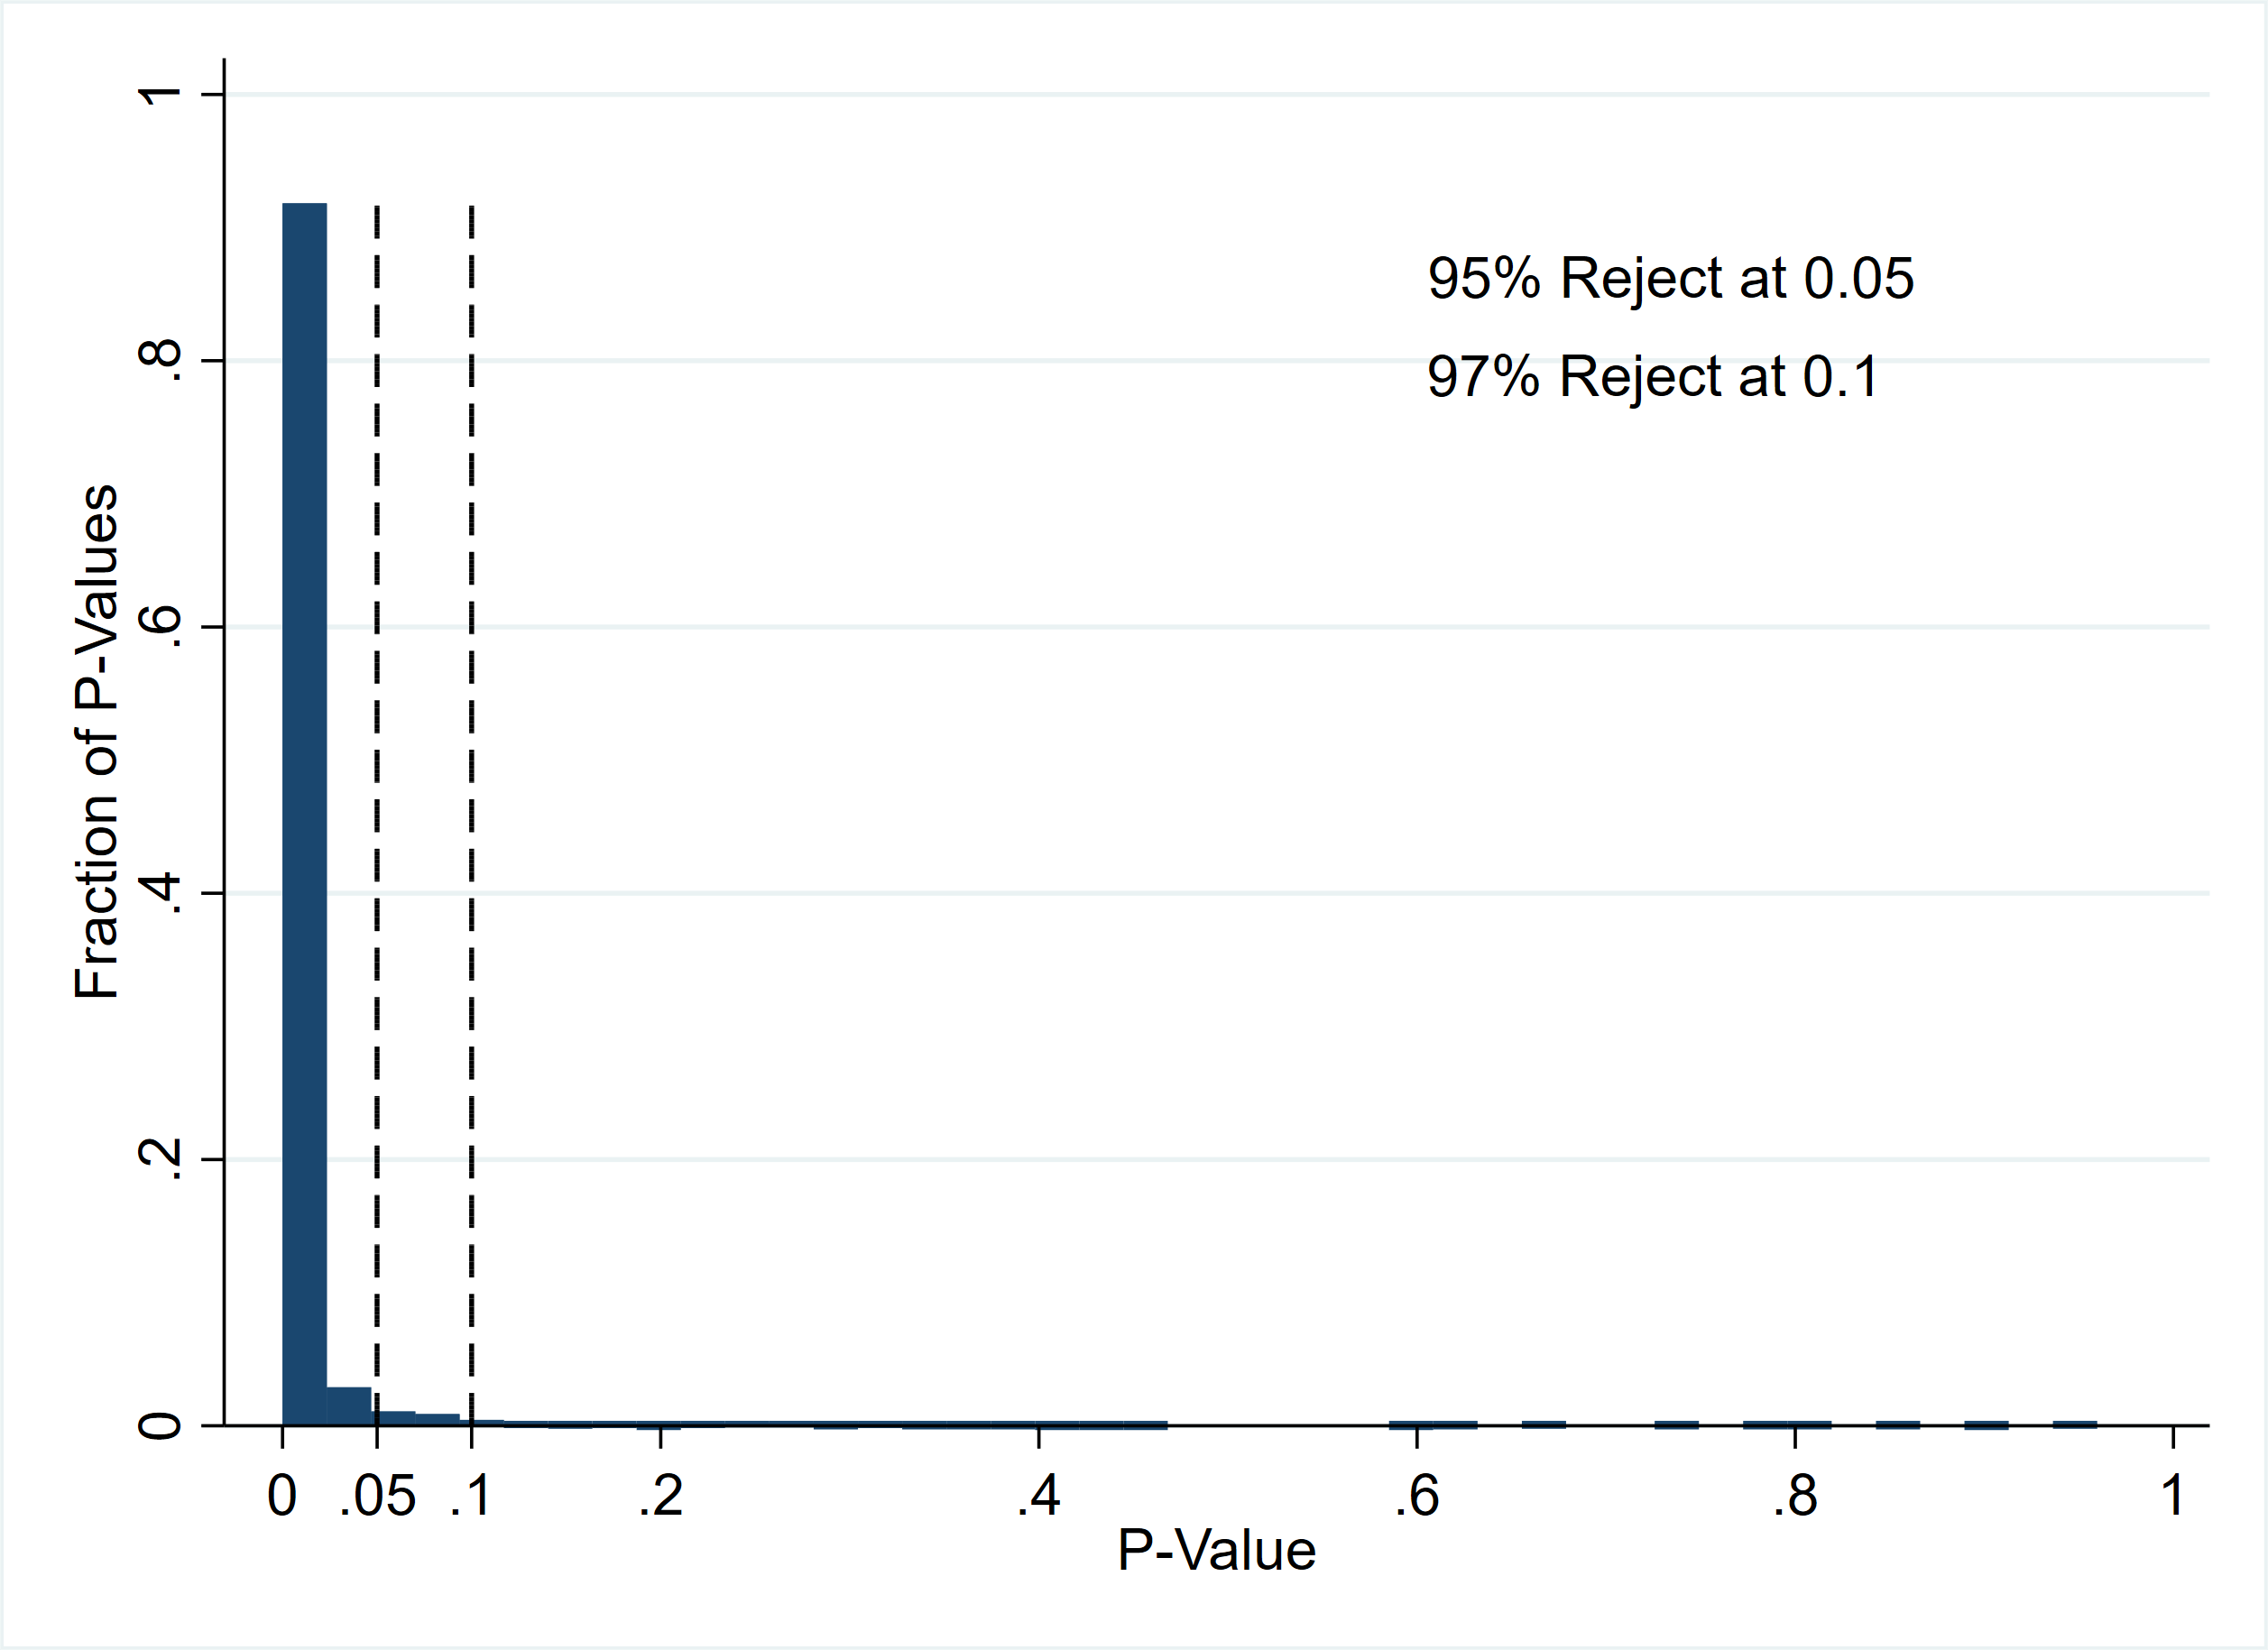
\includegraphics[width=\textwidth]{figures/Math_T_Test_Hist.png}
    \label{fig: math ttest}
\end{figure}

Furthermore, we also categorize teachers where we do or do not find significant differences across the low and high bins by whether the low bin is bigger or the high bin is bigger. This split is shown in Tables \ref{tab: ELA within} and \ref{tab: math within}.

\begin{table}[ht]
    \centering
    \caption{Fraction of Significant Results by Relatively Larger Bin for ELA Value Added Estimates}
    \input{"tables/Within Teacher Test ELA"}
    \label{tab: ELA within}
    \caption*{\scriptsize \textit{Notes:} Results for t-test of hypothesis ``low bin ELA VA estimate = high bin ELA VA estimate'' for each teacher. ``High'' and ``Low'' refer to the estimates for the associated bins.}
\end{table}


\begin{table}[ht]
    \centering
    \caption{Fraction of Significant Results by Relatively Larger Bin for Math Value Added Estimate}
    \input{"tables/Within Teacher Test Math"}
    \label{tab: math within}
    \caption*{\scriptsize \textit{Notes:} Results for t-test of hypothesis ``low bin Math VA estimate = high bin Math VA estimate'' for each teacher. ``High'' and ``Low'' refer to the estimates for the associated bins.}
\end{table}

These results give several broad conclusions. First, we observe substantial heterogeneity within teachers across the two bins. Second, it is not the case that all teachers are better at teaching high achieving students or all are better at teaching low achieving students. If all teachers were better at one and not the other it would suggest either that there are few gains to be made by measuring this heterogeneity because standard value added would handle the level differences between teachers quite well, or it could suggest that the model is wrong and not measuring true heterogeneity. We find that more teachers are better at teaching high achieving students, but a non-trivial minority are relatively better at teaching low achieving students. This suggests that there are possible `gains to trade', meaning that re-arranging students to improve match quality is a possibility.




%%%%%%%%%%%%%%%%%%%%%%%%%%%%%%%%%%%%%%%%%%%%%%%%%%%%%%%%%%%%%%%%%%
%%%%%%%%%%%%%%%%%%%%%%%%%%%%%%%%%%%%%%%%%%%%%%%%%%%%%%%%%%%%%%%%%%
\subsection{Long-Run Outcomes}

Though our simulations and results on within-teacher heterogeneity provide some reassurance that our two-bin VAM is performing reasonably well, the question remains as to whether we are picking up something real with or if the observed differences in standard mean VAM and the two-bin VAM are just noise. To address this questions, we estimate the following equation:

    \begin{equation}\label{eq: standard long run}
        outcome_{it} = \beta_1 VA_{j(i,t)t} + \sum_{i=1}^{10} \mathbbm{1}\{y_{i,t-1} \in decile_i\} + \delta X_{it} + \varepsilon_{it}
    \end{equation}
    
\noindent where $outcome_{it}$ is one of `graduated high school', `enrolled in any college within 1 year of high school', `enrolled in a 2 year college within 1 year of high school', `enrolled in a 4 year college within 1 year of high school', or `earned a Bachelor's degree within 6 years of high school'; $VA_{j(i,t)t}$ is the estimated mean value added in either English language or math for the teacher that the student has in the given year; $\mathbbm{1}\{y_{i,t-1} \in decile_i\}$ is an indicator for decile of achievement based on prior year test score; and $X_{it}$ is a vector of other controls, including lagged average same subject test score for school and classroom, whether the student was ever an English learner or special ed, and year, grade, race, and gender fixed effects. Our standard errors are clustered at the school level. We estimate this equation as a first pass in the spirit of \cite{chetty2014measuring2} to show that we observe similar results to what the authors show in their paper. We are interested in the coefficient on $VA_{j(i,t)t}$, $\beta_1$, which gives the association between a teacher with higher standard value added and the long-run outcomes. Once we have established this, we estimate the following:

    \begin{gather}
        outcome_{it} = \sum_{k=low,high}\left(\beta_{1,k} VA^{low}_{j(i,t)t}*\mathbbm{1}\{y_{i,t-1} \in bin_k\} + \beta_{2,k} VA^{high}_{j(i,t)t}*\mathbbm{1}\{y_{i,t-1} \in bin_k\}\right)\nonumber \\ + \sum_{i=1}^{10} \mathbbm{1}\{y_{i,t-1} \in decile_i\} + \delta X_{it} + \varepsilon_{it}\label{eq: two-bin long run}
    \end{gather}
    
\noindent where $VA^{low/high}_{j(i,t)t}$ is the estimated low/high bin value added in either English language or math for the teacher that the student has in the given year and $\mathbbm{1}\{y_{i,t-1} \in bin_k\}$ is an indicator for whether the student's prior year test score was above (high) or below (low) median in the distribution of prior year test scores. All else is as in described above for equation \ref{eq: standard long run}. Now the interaction terms between the teacher's bin value added and the student's prior achievement bin give us the 4 coefficients of interest, $\beta_{1,low}$, $\beta_{1,high}$, $\beta_{2,low}$, and $\beta_{2,high}$. We interpret $\beta_{1,low}$ and $\beta_{2,high}$ as the `match' effect between a teacher who is particularly good at teaching students that look like the one in question, and the other two coefficients, $\beta_{1,high}$ and $\beta_{2,low}$, as `cross' effects, i.e. all else equal, how is having a teacher good at teaching other students associated with a particular student's long-term outcomes.

Tables \ref{tab:ELA longterm} and \ref{tab:math longterm} show the results of using our estimates (scaled by the standard deviation of teacher estimates) to predict long-term outcomes.

\begin{landscape}
    \vspace*{\fill}
    \begin{table}[ht]
        \centering
        \caption{Long-Term Outcomes by ELA Value Added Estimates}
        \resizebox{1.4\textwidth}{!}{\input{"tables/Long Term Outcomes ELA"}}
        \label{tab:ELA longterm}
    \end{table}
    \centering
    \footnotesize{\textit{Notes:} Standard Errors in parentheses. *** $p<0.01$, ** $p<0.05$, * $p<0.1$. The outcomes are the following: `Graduated High School' is an indicator for whether the student graduated from high school, `Enrolled in Any College' is an indicator for whether the student enrolled in any type of college within a year following high school, `Enrolled in 2yr College' is an indicator for whether the student enrolled in a 2 year college within a year following high school, `Enrolled in 4yr College' is an indicator for whether the student enrolled in a 4 year college within a year following high school, and `Graduated w/ Bachelor's' is an indicator for whether the student earned a Bachelor's degree within 6 years of high school. Odd columns reflect estimates of standard ELA value added from equation \ref{eq: standard}, even columns reflect estimates of two-bin ELA value added from equation \ref{eq: bins}.}
    \vspace*{\fill}
\end{landscape}

\begin{landscape}
    \vspace*{\fill}
    \begin{table}[ht]
        \centering
        \caption{Long-Term Outcomes by Math Value Added Estimates}
        \resizebox{1.4\textwidth}{!}{\input{"tables/Long Term Outcomes Math"}}
        \label{tab:math longterm}
    \end{table}fh
    \centering
    \footnotesize{\textit{Notes:} Standard Errors in parentheses. *** $p<0.01$, ** $p<0.05$, * $p<0.1$. The outcomes are the following: `Graduated High School' is an indicator for whether the student graduated from high school, `Enrolled in Any College' is an indicator for whether the student enrolled in any type of college within a year following high school, `Enrolled in 2yr College' is an indicator for whether the student enrolled in a 2 year college within a year following high school, `Enrolled in 4yr College' is an indicator for whether the student enrolled in a 4 year college within a year following high school, and `Graduated w/ Bachelor's' is an indicator for whether the student earned a Bachelor's degree within 6 years of high school. Odd columns reflect estimates of standard Math value added from equation \ref{eq: standard}, even columns reflect estimates of two-bin Math value added from equation \ref{eq: bins}.}
    \vspace*{\fill}
\end{landscape}

Similar to the results presented in \cite{chetty2014measuring2}, our standard value added estimates in ELA and math are strongly predictive of graduating high school, enrolling in college within a year of high school, and graduating with a Bachelor's degree within 6 years of high school. In particular, the results in odd numbered columns show that students who have teacher with 1 sd higher mean value added in ELA at 1 pp more likely to graduate from high school, 1.2 pp more likely to enroll in any college, 0.9 pp less likely to enroll in a 2 year college, 2.1 pp more likely to enroll in a 4 year college, and 1.5 pp more likely to graduate with a Bachelor's degree within 6 years of high school. Results are qualitatively similar (though a bit smaller in magnitude) for teachers with higher standard value added in math.

More interesting, though, are the results presented in the even columns of tables \ref{tab:ELA longterm} and \ref{tab:math longterm} for estimates of equation \ref{eq: two-bin long run}. A strong pattern emerges for the `match' effect between high below median value added teachers and below median students as well as for high above median value added teachers and above median students. Importantly, as we interpret these results we need to consider which students are on the margin for each outcome. Though students at any point in the prior achievement distribution can certainly be on the margin for any of our long-term outcomes, on average each of the outcomes is increasing throughout the prior test score distribution, with the exception of `2 year college enrollment' which peaks around the 30th percentile and declines thereafter. High school graduation rates steeply rise until around the 30th percentile, around which they level off. All other outcomes are most steeply rising in the top half of the distribution. Based on this we might expect that the majority of `compliers' for these high school graduation would be in the bottom half of the distribution, throughout for enrolling in a 2 year college, and in the top half of the distribution for the other outcomes.

Throughout the following paragraphs we report the results for ELA with those for math in parentheses. We also refer to match and cross effects by saying, for example, below/below for a teacher with high below median value added with a student below the median. Thus when we say, for example, that the above/above match effect for the outcome was 2 pp, we mean that a student who has an above median prior test score and is taught by a teacher with a 1 sd higher above median value added is 2 pp more likely to have that outcome. 

Our results are roughly consistent with the broad observations from the previous paragraph. The result that is most in conflict with these priors is for high school graduation, where we see a significant but modest above/above match effect of 0.8 (0.7) pp. The below/below match effect is of similar magnitude, but noisier and thus insignificant.

Outside of the high school graduation results, the observed match effects are consistent with the priors derived from which students are likely to be compliers from the raw data. We observe below/below and above/above match effects for any college enrollment of 1.5 (0.5) pp and 1.6 (1.7) pp respectively. Once we break this down into 2 year and 4 year enrollment we see that below/below match effects more strongly move students into 2 year college (a significant ELA result of 1 (-.3) pp increase) while above/above match effects pull seem to move students from enrolling in 2 year colleges (-2.4 (-1.1) pp) and push them to enroll in 4 year colleges (4.5 (3.1) pp). Furthermore, the above/above match effect for earning a Bachelor's degree is 3.3 (2.6) pp, while there is no significant below/below effect.

Results with the cross effects are more mixed, but are primarily insignificant and negative. This suggests that, all else equal, a student in a class with a teacher who is better at teaching other students either is equally well off or experiences a slight decrease in their long-term outcomes.

Overall these results are strong evidence of match effects between teachers and students. They also show that the heterogeneity we are picking up matters for real-world outcomes rather and is thus unlikely to just be noise.




%%%%%%%%%%%%%%%%%%%%%%%%%%%%%%%%%%%%%%%%%%%%%%%%%%%%%%%%%%%%%%%%%%
%%%%%%%%%%%%%%%%%%%%%%%%%%%%%%%%%%%%%%%%%%%%%%%%%%%%%%%%%%%%%%%%%%
%%%%%%%%%%%%%%%%%%%%%%%%%%%%%%%%%%%%%%%%%%%%%%%%%%%%%%%%%%%%%%%%%%
\section{Are Standard Value Added Measures Regressive?}\label{sec: Regressive VA}

%%%%%%%%%%%%%%%%%%%%%%%%%%%%%%%%%%%%%%%%%%%%%%%%%%%%%%%%%%%%%%%%%%
%%%%%%%%%%%%%%%%%%%%%%%%%%%%%%%%%%%%%%%%%%%%%%%%%%%%%%%%%%%%%%%%%%
\subsection{Value Added Breaks In the Presence of Heterogeneity}

Now we examine the induced weighting brought on by standard value added estimates. Figures \ref{fig: ELA resid Naive} and \ref{fig: Math resid Naive} shows the average residuals from the naive, simple regression of test scores on once lagged test scores. A strong pattern emerges (outside of the tails of the distribution) where students above the median in the past year test score distribution (roughly) have large, positive residuals and those below the median have large negative residuals. However, this is not necessarily problematic for standard value added estimates. If teachers have homogeneous effects along the achievement distribution and teachers all have a uniform distribution of students, then standard value added estimates will rank teachers correctly. In practice, though, students are sorted (to a greater or lesser extent into classes). We show some evidence of this in the SDUSD data in Section \ref{sec: Robust} Furthermore, given our results from the prior section, it is also not true that teachers have homogeneous effects along the achievement distribution. 

These things together imply that standard value added estimates will give more credit to teachers who (1) teach more high achieving students and (2) have higher value added for high achieving students. In terms of our simple framework given in equation \ref{eq: welfare}, the explicit weights for standard value added are equal for each student ($\omega(y_{i,t-1}, x_{it}) = 1/N_j$). However, the estimated value, $\hat{v}(y_{it}, y_{i,t-1}, x_{it})$, is too high for high achieving students and too low for low achieving students.

\begin{figure}[ht]
    \centering
    \caption{Naive ELA Regression Residuals}
    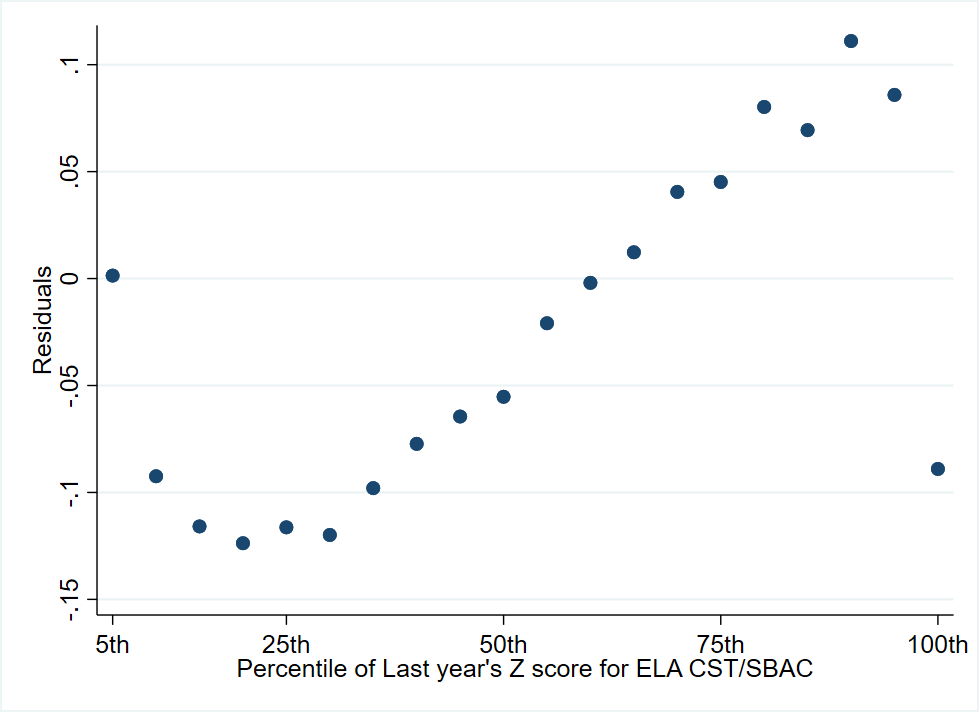
\includegraphics[width=\textwidth]{figures/ELA_Resid_Naive.png}
    \label{fig: ELA resid Naive}
\end{figure}

\begin{figure}[ht]
    \centering
    \caption{Naive Math Regression Residuals}
    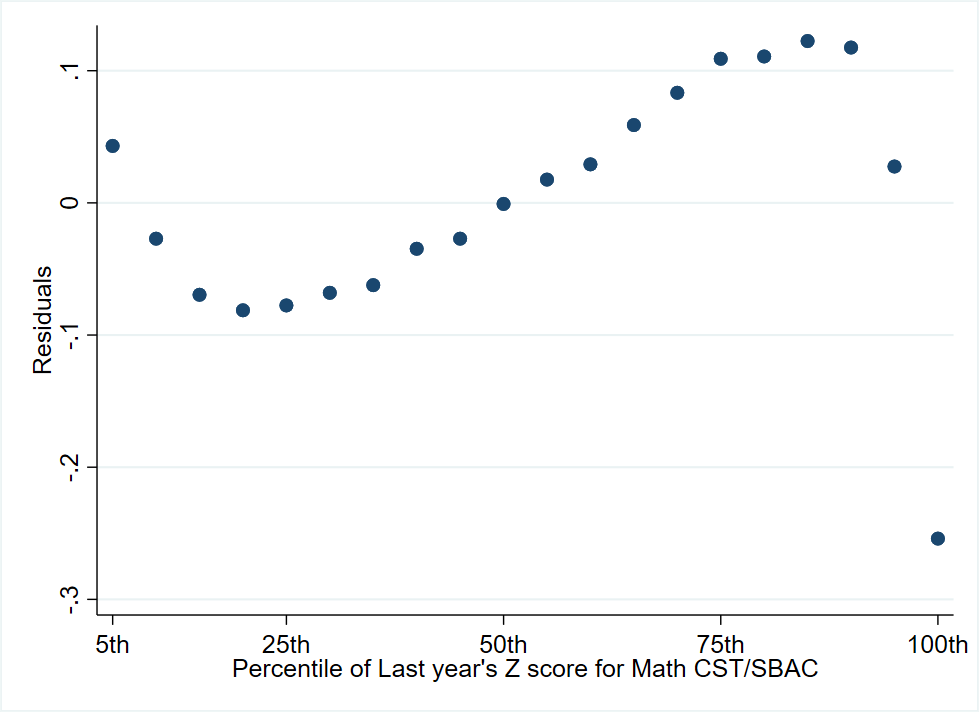
\includegraphics[width=\textwidth]{figures/Math_Resid_Naive.png}
    \label{fig: Math resid Naive}
\end{figure}

Very few, if any, reasonable researchers or policymakers rely on the simple regression of test scores on lagged test scores when calculating standard value added for teachers. We thus run our preferred specification from equation \ref{eq: standard} and show the results in Figures \ref{fig: ELA resid Preferred} and \ref{fig: Math resid Preferred}. The magnitude of the disparity between residuals below and above the mean shrinks considerably, but the strong pattern previously observed remains. Furthermore, if we run our preferred specification plus a cubic in past test scores and school fixed-effects the residuals in Figure \ref{fig: ELA resid Everything} and \ref{fig: Math resid Everything} reflect the very same pattern, though the magnitude is once again significantly smaller.

\begin{figure}[ht]
    \centering
    \caption{Preferred ELA Regression Residuals}
    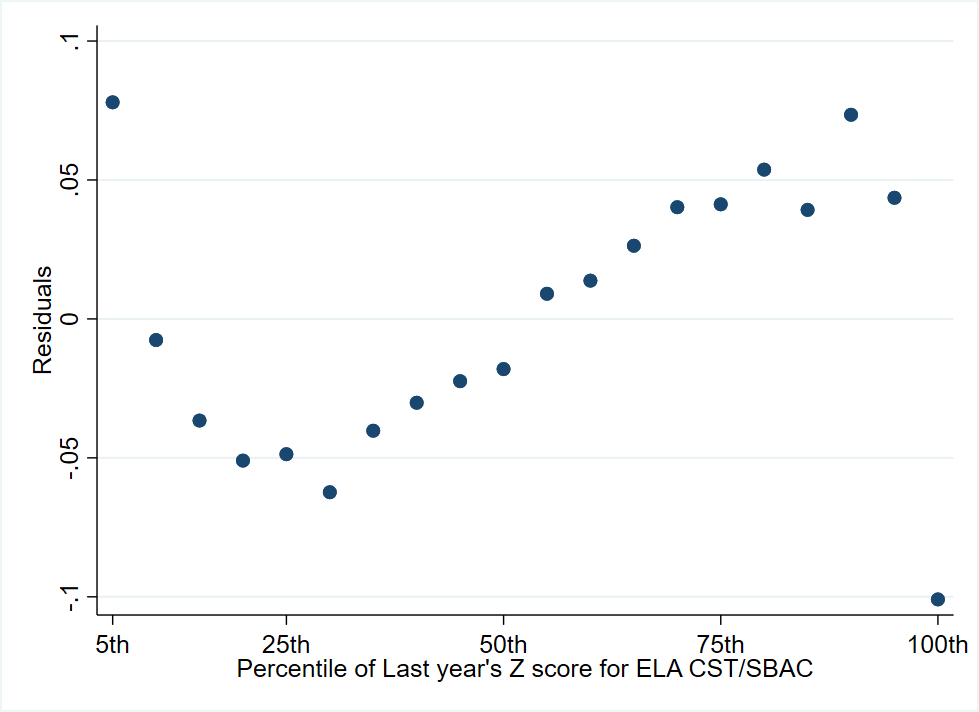
\includegraphics[width=\textwidth]{figures/ELA_Resid_Preferred.png}
    \label{fig: ELA resid Preferred}
\end{figure}

\begin{figure}[ht]
    \centering
    \caption{Preferred Math Regression Residuals}
    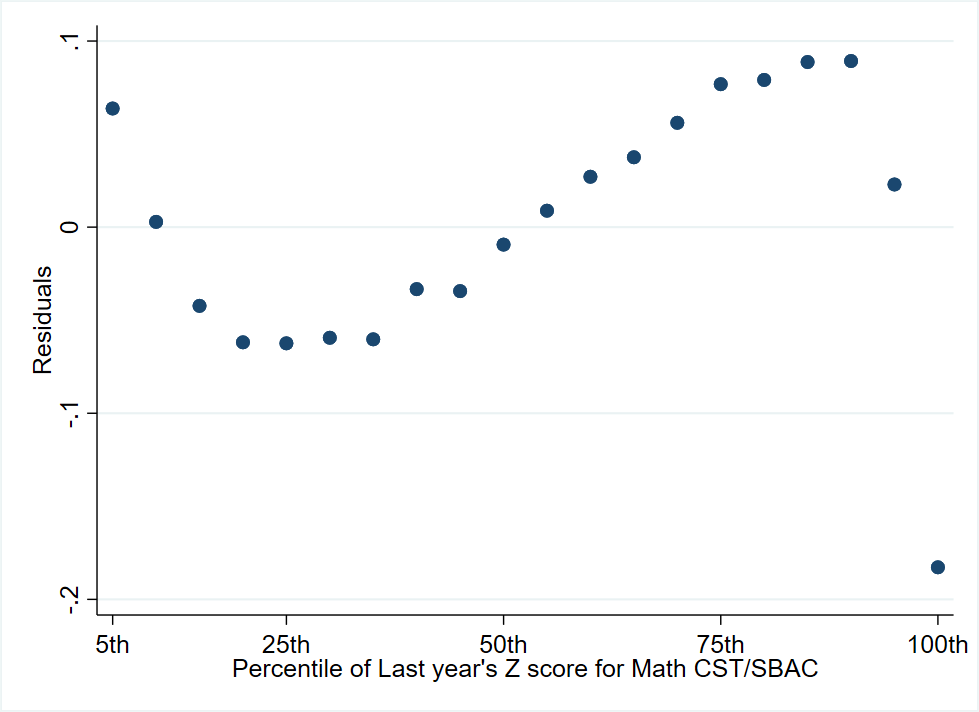
\includegraphics[width=\textwidth]{figures/Math_Resid_Preferred.png}
    \label{fig: Math resid Preferred}
\end{figure}

\begin{figure}[ht]
    \centering
    \caption{Everything ELA Regression Residuals}
    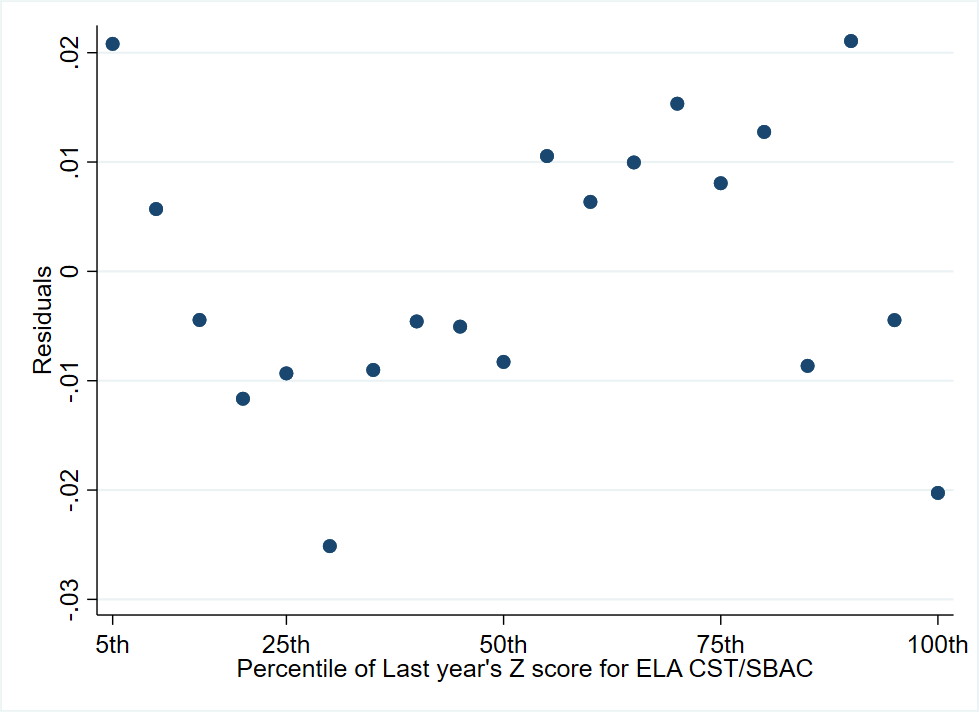
\includegraphics[width=\textwidth]{figures/ELA_Resid_Everything.png}
    \label{fig: ELA resid Everything}
\end{figure}

\begin{figure}[ht]
    \centering
    \caption{Everything Math Regression Residuals}
    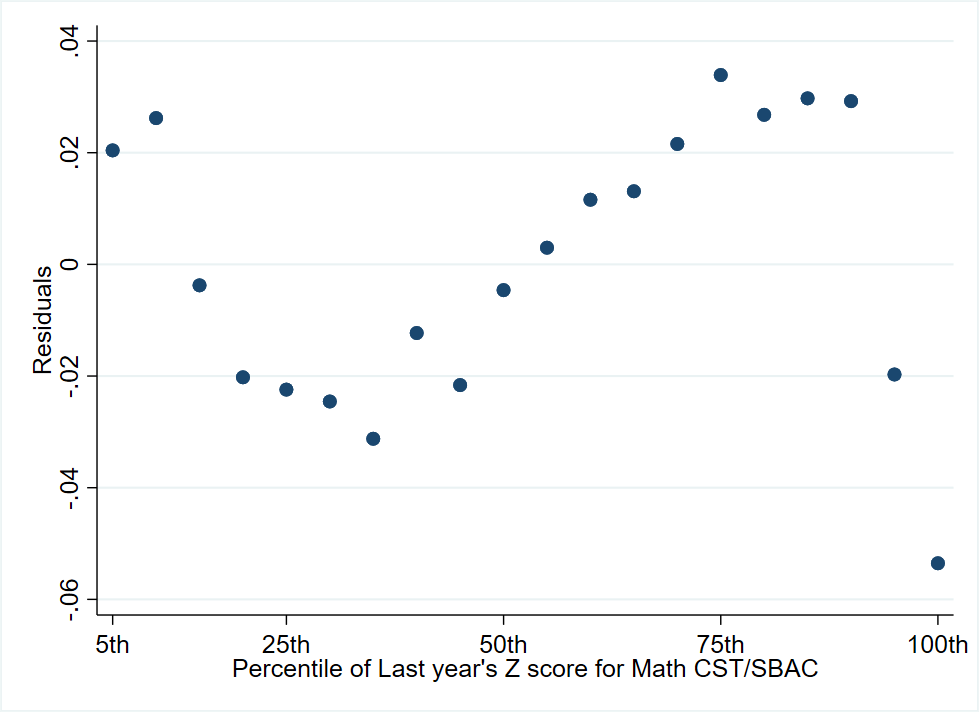
\includegraphics[width=\textwidth]{figures/Math_Resid_Everything.png}
    \label{fig: Math resid Everything}
\end{figure}

This is problematic given our findings of heterogeneity. In particular, this implies that standard value added estimates do not produce a desirable, utilitarian weighting that seems to intuitively come from using them. They rather produce a regressive weighting, putting more weight on high achieving students when we are measuring how much value teachers are contributing to their students, which is entirely counter to the stated goals of many education policies.



%%%%%%%%%%%%%%%%%%%%%%%%%%%%%%%%%%%%%%%%%%%%%%%%%%%%%%%%%%%%%%%%%%
%%%%%%%%%%%%%%%%%%%%%%%%%%%%%%%%%%%%%%%%%%%%%%%%%%%%%%%%%%%%%%%%%%
% \subsection{Implications for Minority Teachers}



%%%%%%%%%%%%%%%%%%%%%%%%%%%%%%%%%%%%%%%%%%%%%%%%%%%%%%%%%%%%%%%%%%
%%%%%%%%%%%%%%%%%%%%%%%%%%%%%%%%%%%%%%%%%%%%%%%%%%%%%%%%%%%%%%%%%%
\subsection{Policy Applications of Flexible Value Added}

Though more work remains to understand and quantify the actionable conclusions of this work, we provide a few suggestions of possible policy applications to our work. Similar to \cite{condie2014teacher}, one important possibility is that of matching teachers with students based on comparative advantage. Due to union and feasibility constraints, there are really only three plausible reassignment policies. First, leaving teachers fixed within schools and shuffling students across teachers within the same school. This is by far the most reasonable reassignment policy. Another possibility is leaving students fixed and reassigning teachers within a school. These both provide potential gains to students with very little cost.

Another attractive application for the work we have done here is using the estimates to identify teachers who are particularly succeeding or struggling to push forward the district or state's distributional goals for training or incentive purposes.

These are just a few suggestions for possible policy applications, much more work is needed to fill these in.
 



%%%%%%%%%%%%%%%%%%%%%%%%%%%%%%%%%%%%%%%%%%%%%%%%%%%%%%%%%%%%%%%%%%
%%%%%%%%%%%%%%%%%%%%%%%%%%%%%%%%%%%%%%%%%%%%%%%%%%%%%%%%%%%%%%%%%%
%%%%%%%%%%%%%%%%%%%%%%%%%%%%%%%%%%%%%%%%%%%%%%%%%%%%%%%%%%%%%%%%%%
% \section{Extensions to More Flexible Heterogeneity}\label{sec: Extensions}

% Teaser section about using the nonparametric kernel regression.




%%%%%%%%%%%%%%%%%%%%%%%%%%%%%%%%%%%%%%%%%%%%%%%%%%%%%%%%%%%%%%%%%%
%%%%%%%%%%%%%%%%%%%%%%%%%%%%%%%%%%%%%%%%%%%%%%%%%%%%%%%%%%%%%%%%%%
%%%%%%%%%%%%%%%%%%%%%%%%%%%%%%%%%%%%%%%%%%%%%%%%%%%%%%%%%%%%%%%%%%
\section{Robustness Checks}\label{sec: Robust}

%%%%%%%%%%%%%%%%%%%%%%%%%%%%%%%%%%%%%%%%%%%%%%%%%%%%%%%%%%%%%%%%%%
%%%%%%%%%%%%%%%%%%%%%%%%%%%%%%%%%%%%%%%%%%%%%%%%%%%%%%%%%%%%%%%%%%
\subsection{Classroom Sorting}

As we build more flexibility into our value added estimates, we very quickly run into a support problem. Conceptually, if we had infinite students per teacher we could estimate value added at each point in the prior year test score distribution. Given reasonable data limitations, though, a reasonable concern is to what extent we have problems with support in estimating flexible value added. Given our original simulation results, we limited the analysis to teachers who had a minimum of 50 students with consecutive years of test scores. Figures \ref{fig: ELA sort 2 50}-\ref{fig: ELA sort 4 200} give the fraction of students who fall in a teachers smaller bin when we split the students into above and below median bins by prior year ELA test score (see Figures \ref{fig: Math sort 2 50}-\ref{fig: Math sort 4 200} for the corresponding Math test score figures). For example, a teacher who taught 30 students below the median and 70 students above would have 30\% of her students in the smallest bin.

Figure \ref{fig: ELA sort 2 50} shows that despite just using two-bins, we are still unable to estimate one of the two bins for 14\% of teachers. Once we limit to 200 students per teacher, however, the problem is substantially reduced (see Figure \ref{fig: ELA sort 2 200}). This conclusion also holds for 4 bins.

\begin{figure}[ht]
    \centering
    \caption{Sorting by Prior Year ELA Score with 2 Bins, Min 50 Students per Teacher}
    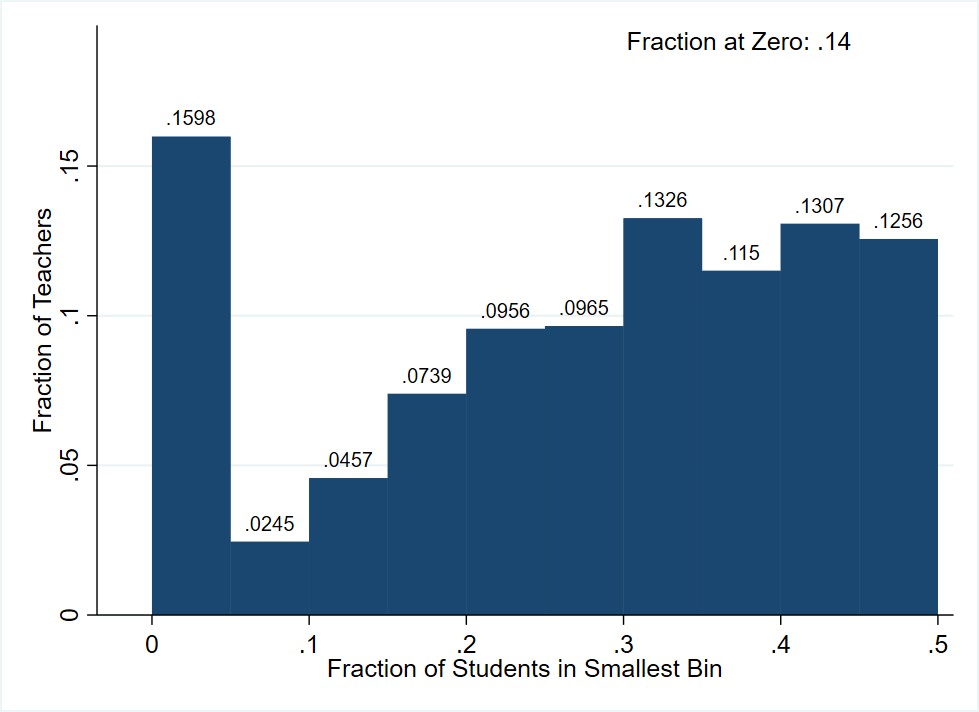
\includegraphics[width=\textwidth]{figures/ELA_Sorting_2_50.png}
    \label{fig: ELA sort 2 50}
\end{figure}

\begin{figure}[ht]
    \centering
    \caption{Sorting by Prior Year ELA Score with 4 Bins, Min 50 Students per Teacher}
    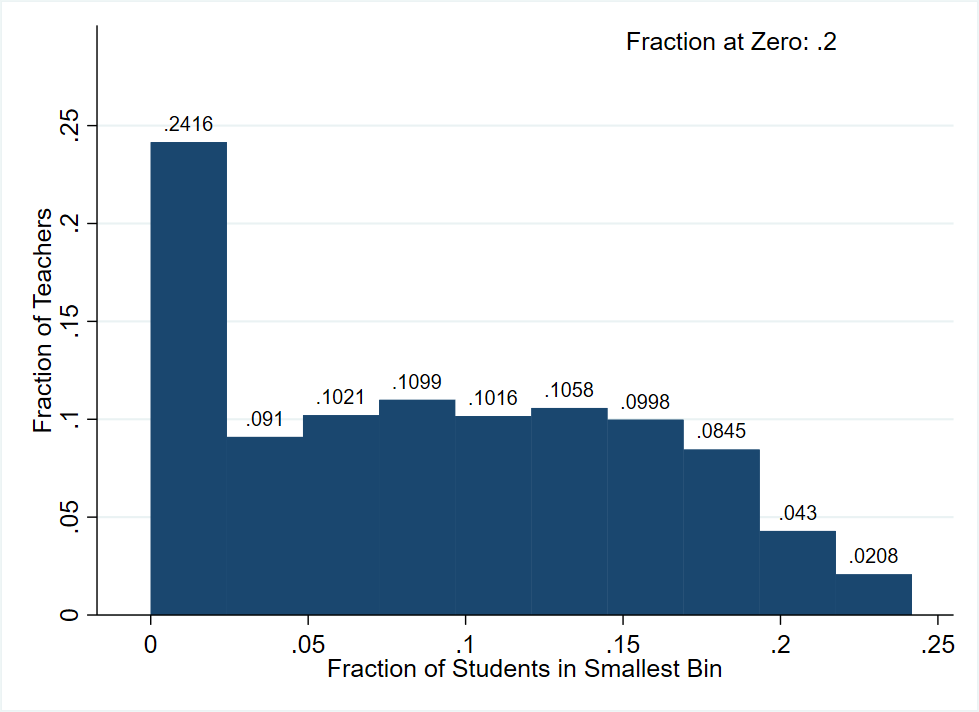
\includegraphics[width=\textwidth]{figures/ELA_Sorting_4_50.png}
    \label{fig: ELA sort 4 50}
\end{figure}

\begin{figure}[ht]
    \centering
    \caption{Sorting by Prior Year ELA Score with 2 Bins, Min 200 Students per Teacher}
    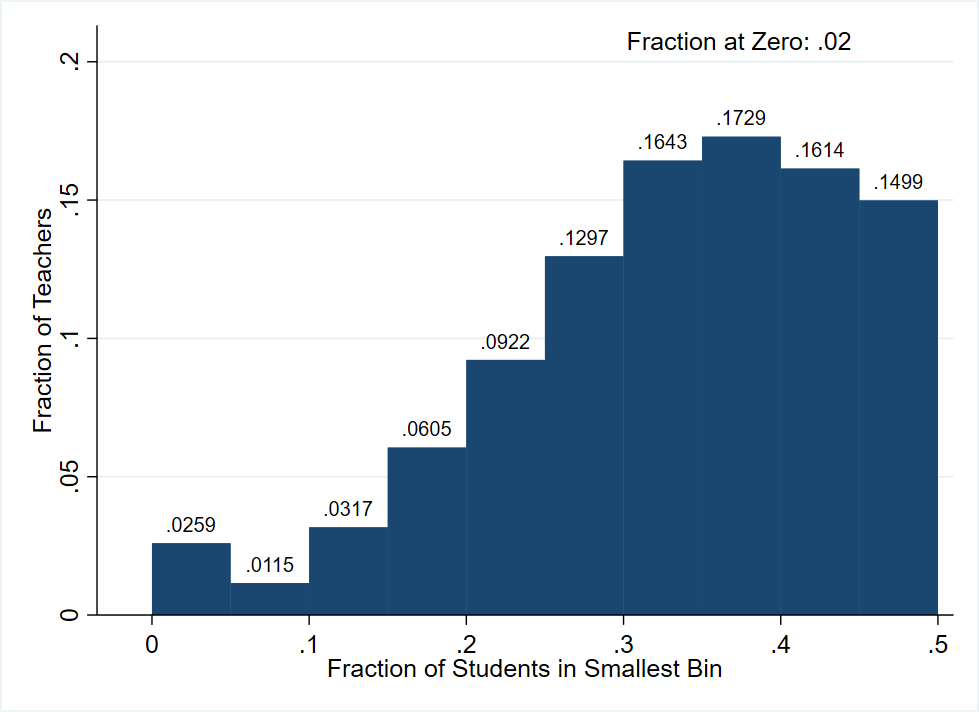
\includegraphics[width=\textwidth]{figures/ELA_Sorting_2_200.png}
    \label{fig: ELA sort 2 200}
\end{figure}

\begin{figure}[ht]
    \centering
    \caption{Sorting by Prior Year ELA Score with 4 Bins, Min 200 Students per Teacher}
    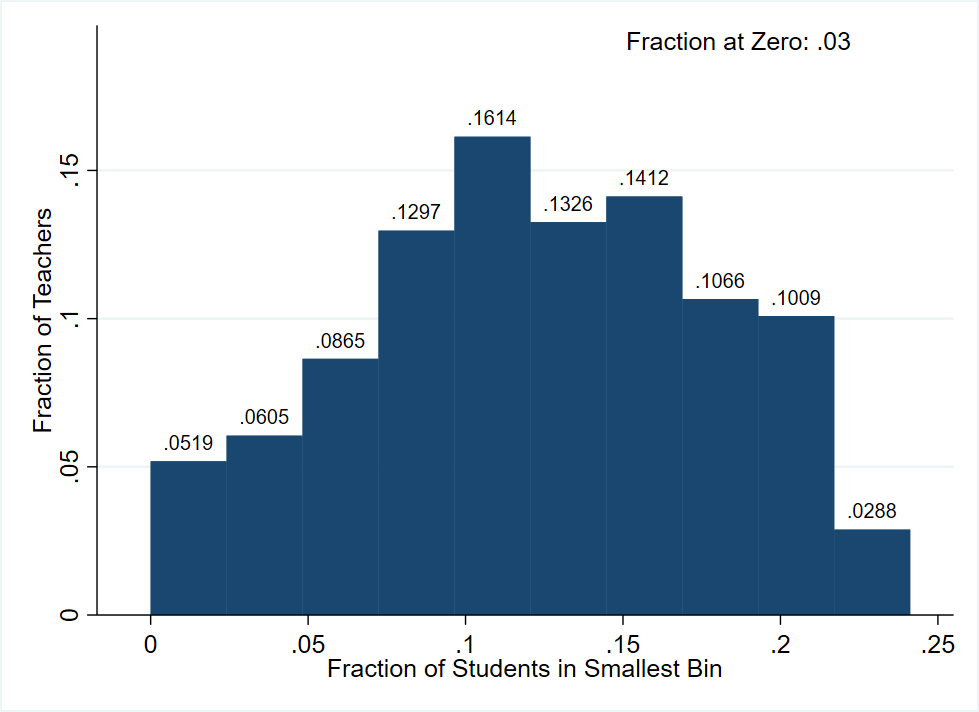
\includegraphics[width=\textwidth]{figures/ELA_Sorting_4_200.png}
    \label{fig: ELA sort 4 200}
\end{figure}

To attempt to speak to the potential problems caused by sorting, we re-run our analyses limiting our sample to teachers who have a minimum of 200 students with consecutive test scores rather than just those with a minimum of 50 students. This substantially limits our sample, but still leaves us with nearly 350 teachers and 18,000 students. When considering the amount of within teacher variation in match quality that exists and the ability of the estimates to predict long-term outcomes, our results are both qualitatively and quantitatively similar. This suggests that teachers with small bins (and thus noisier estimates) are not those driving the results that we observe.



%%%%%%%%%%%%%%%%%%%%%%%%%%%%%%%%%%%%%%%%%%%%%%%%%%%%%%%%%%%%%%%%%%
%%%%%%%%%%%%%%%%%%%%%%%%%%%%%%%%%%%%%%%%%%%%%%%%%%%%%%%%%%%%%%%%%%
% \subsection{Bias of Estimates a la \cite{chetty2014measuring1}}




%%%%%%%%%%%%%%%%%%%%%%%%%%%%%%%%%%%%%%%%%%%%%%%%%%%%%%%%%%%%%%%%%%
%%%%%%%%%%%%%%%%%%%%%%%%%%%%%%%%%%%%%%%%%%%%%%%%%%%%%%%%%%%%%%%%%%
%%%%%%%%%%%%%%%%%%%%%%%%%%%%%%%%%%%%%%%%%%%%%%%%%%%%%%%%%%%%%%%%%%
\section{Conclusion}\label{sec: Conclusion}

Standard value added estimates are becoming increasingly common in evaluating relative teacher performance. However, these are mean oriented statistics and many education policies have distributional goals, so standard value added estimates are not necessarily an appropriate tool to measure and pursue these goals. We argue that standard value added estimates actual induce a regressive weighting over students, giving too much credit to teachers who are especially benefiting high achieving students and visa verso for those particularly helping low achieving students.

We show evidence of heterogeneity in teacher value added across the achievement distribution. Not only do we demonstrate this `match' effect, but we show that this match effect matters for student long-term outcomes, such as graduation from high school, enrolling in college, and graduating with a Bachelor's degree.

Our findings have important implications for policymakers seeking to help particular groups of students. More work is needed to understand whether and to what extent we can estimate increasingly flexible value added measures as well as to explore the interaction between teacher match effects and incentive structures.





%%%%%%%%%%%%%%%%%%%%%%%%%%%%%%%%%%%%%%%%%%%%%%%%%%%%%%%%%%%%%%%%%%
%%%%%%%%%%%%%%%%%%%%%%%%%%%%%%%%%%%%%%%%%%%%%%%%%%%%%%%%%%%%%%%%%%
%%%%%%%%%%%%%%%%%%%%%%%%%%%%%%%%%%%%%%%%%%%%%%%%%%%%%%%%%%%%%%%%%%
\bibliography{citations}




%%%%%%%%%%%%%%%%%%%%%%%%%%%%%%%%%%%%%%%%%%%%%%%%%%%%%%%%%%%%%%%%%%
%%%%%%%%%%%%%%%%%%%%%%%%%%%%%%%%%%%%%%%%%%%%%%%%%%%%%%%%%%%%%%%%%%
%%%%%%%%%%%%%%%%%%%%%%%%%%%%%%%%%%%%%%%%%%%%%%%%%%%%%%%%%%%%%%%%%%
\appendix

\renewcommand\thefigure{\thesection.\arabic{figure}}
\setcounter{figure}{0}  

%%%%%%%%%%%%%%%%%%%%%%%%%%%%%%%%%%%%%%%%%%%%%%%%%%%%%%%%%%%%%%%%%%
%%%%%%%%%%%%%%%%%%%%%%%%%%%%%%%%%%%%%%%%%%%%%%%%%%%%%%%%%%%%%%%%%%
\section{Appendix Figures}\label{sec: Appendix Figures}

\begin{figure}[ht]
    \centering
    \caption{Correlation Between ELA Low Bin and High Bin Estimates}
    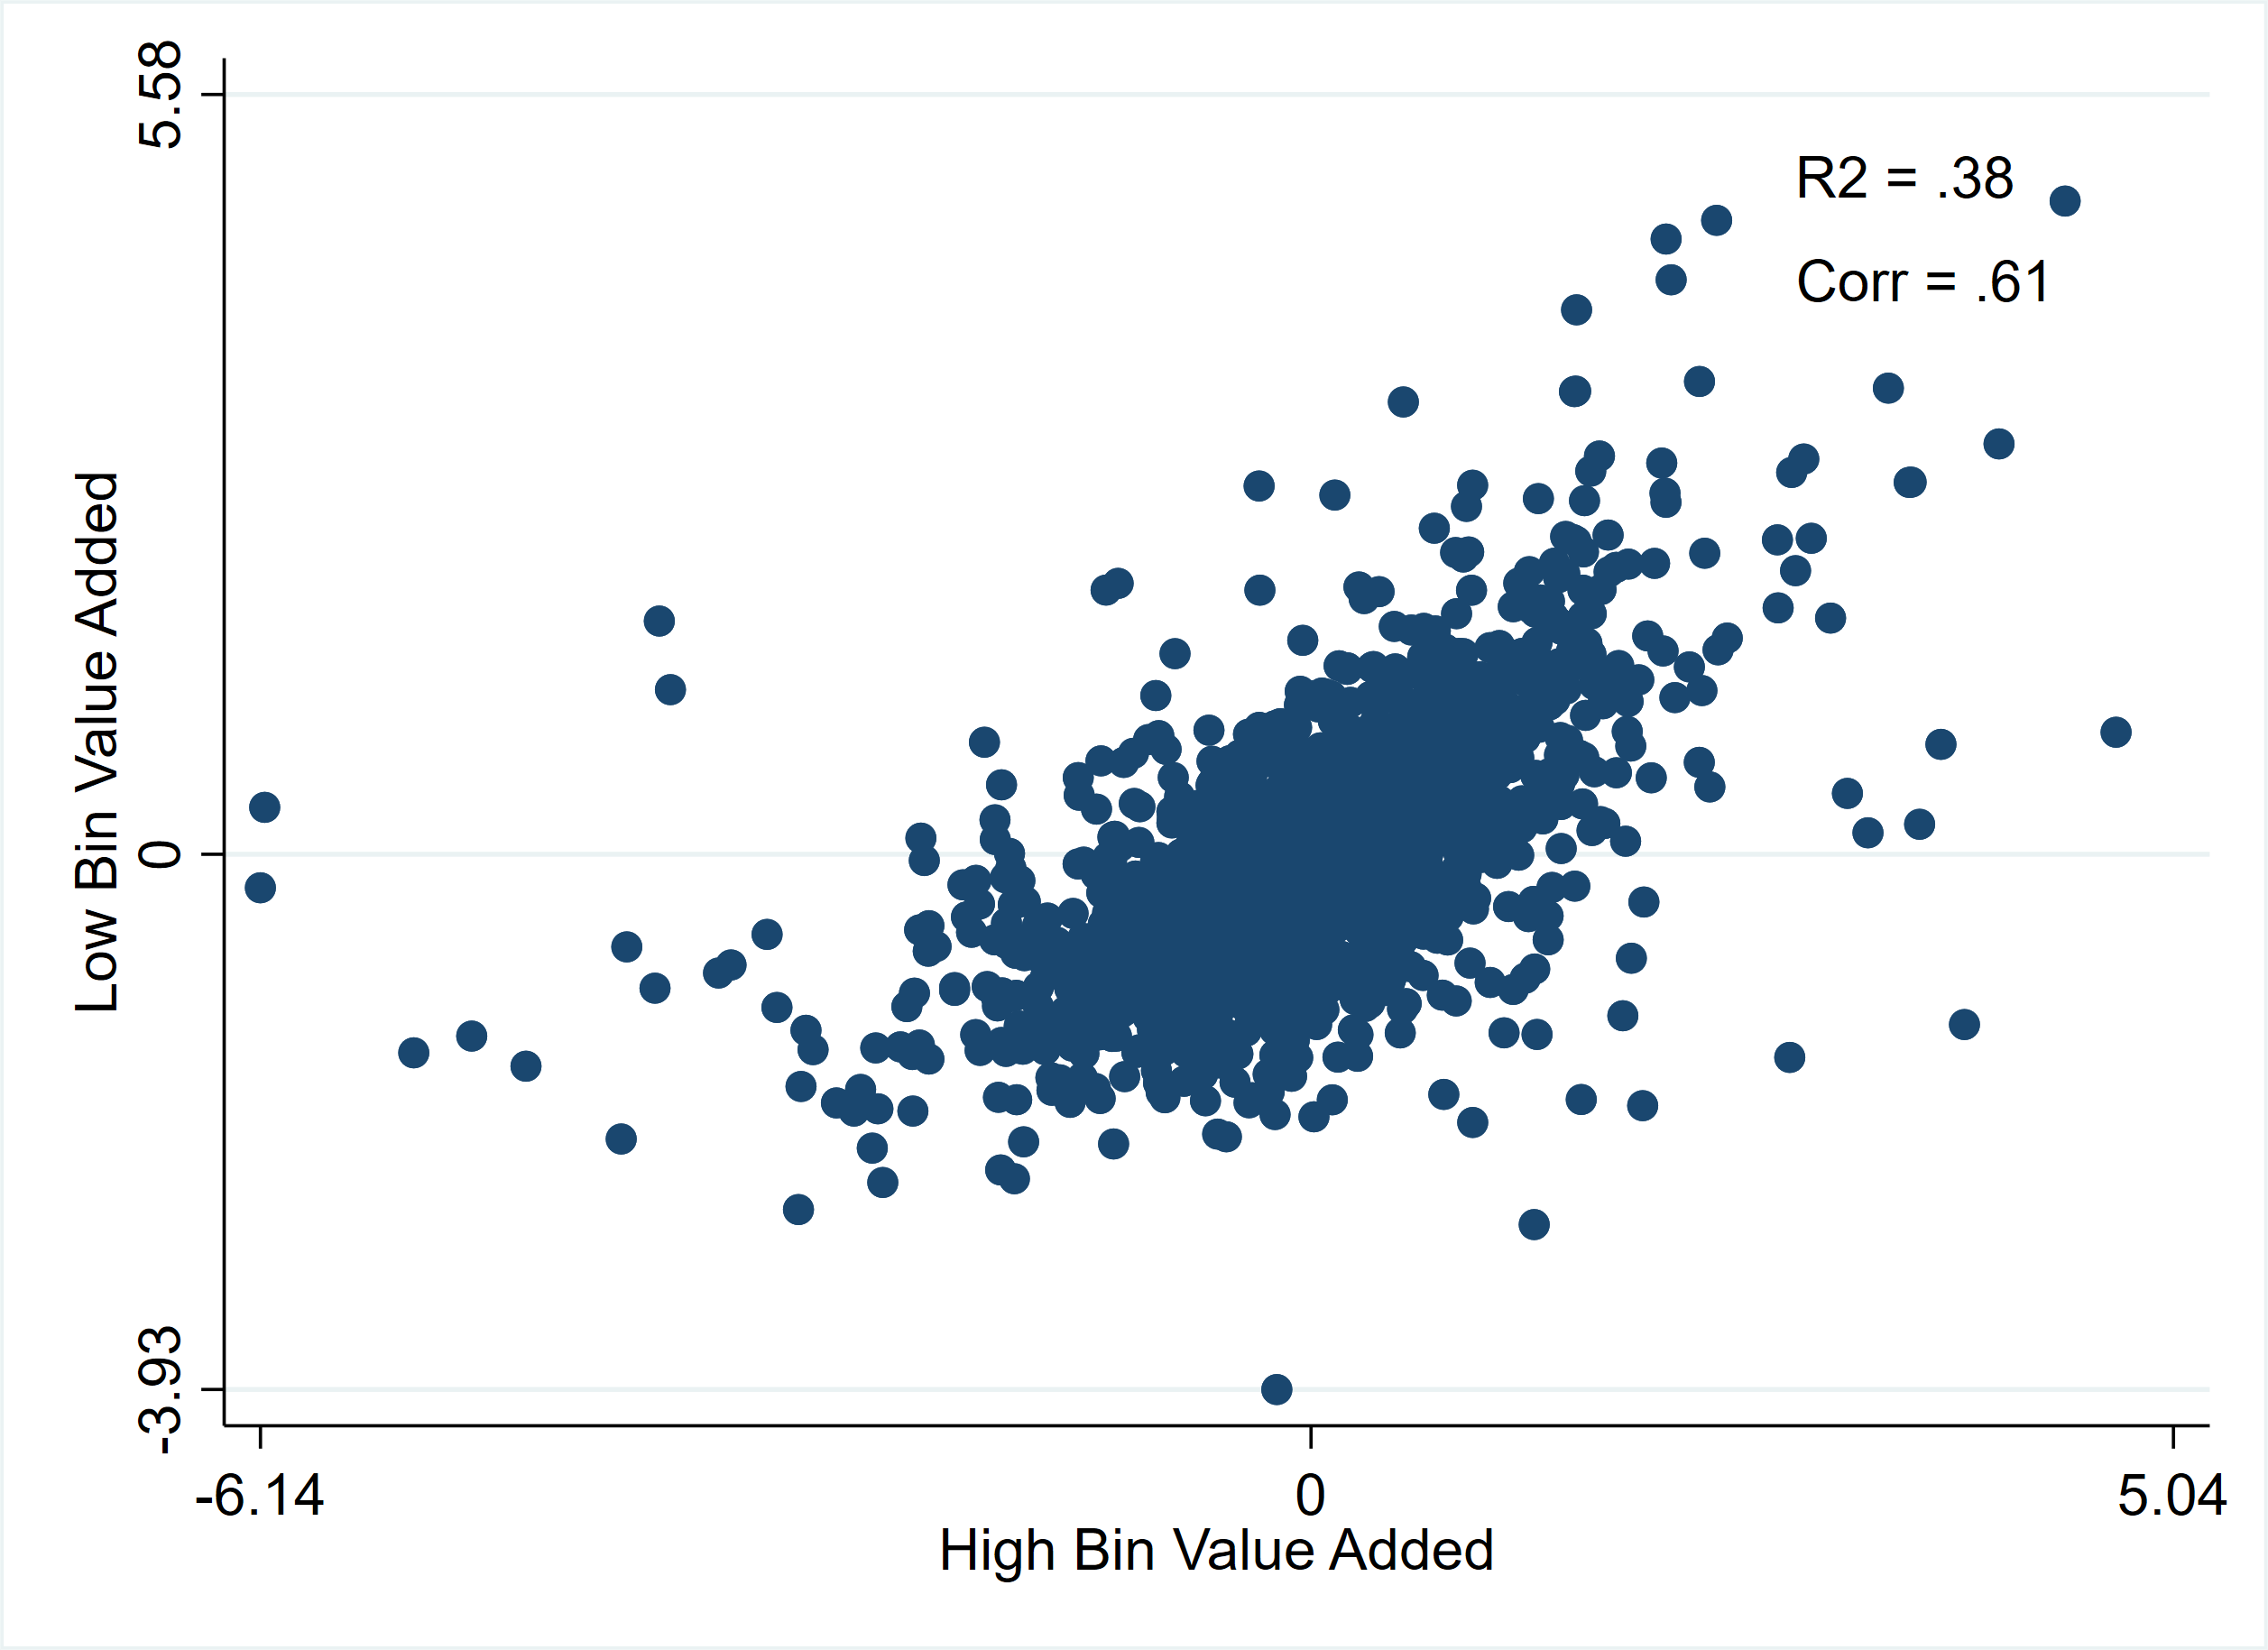
\includegraphics[width=\textwidth]{figures/ELA_High_Bin_Versus_Low_Bin.png}
    \label{fig: ELA corr}
\end{figure}

\begin{figure}[ht]
    \centering
    \caption{Correlation Between ELA Low Bin and High Bin Estimates}
    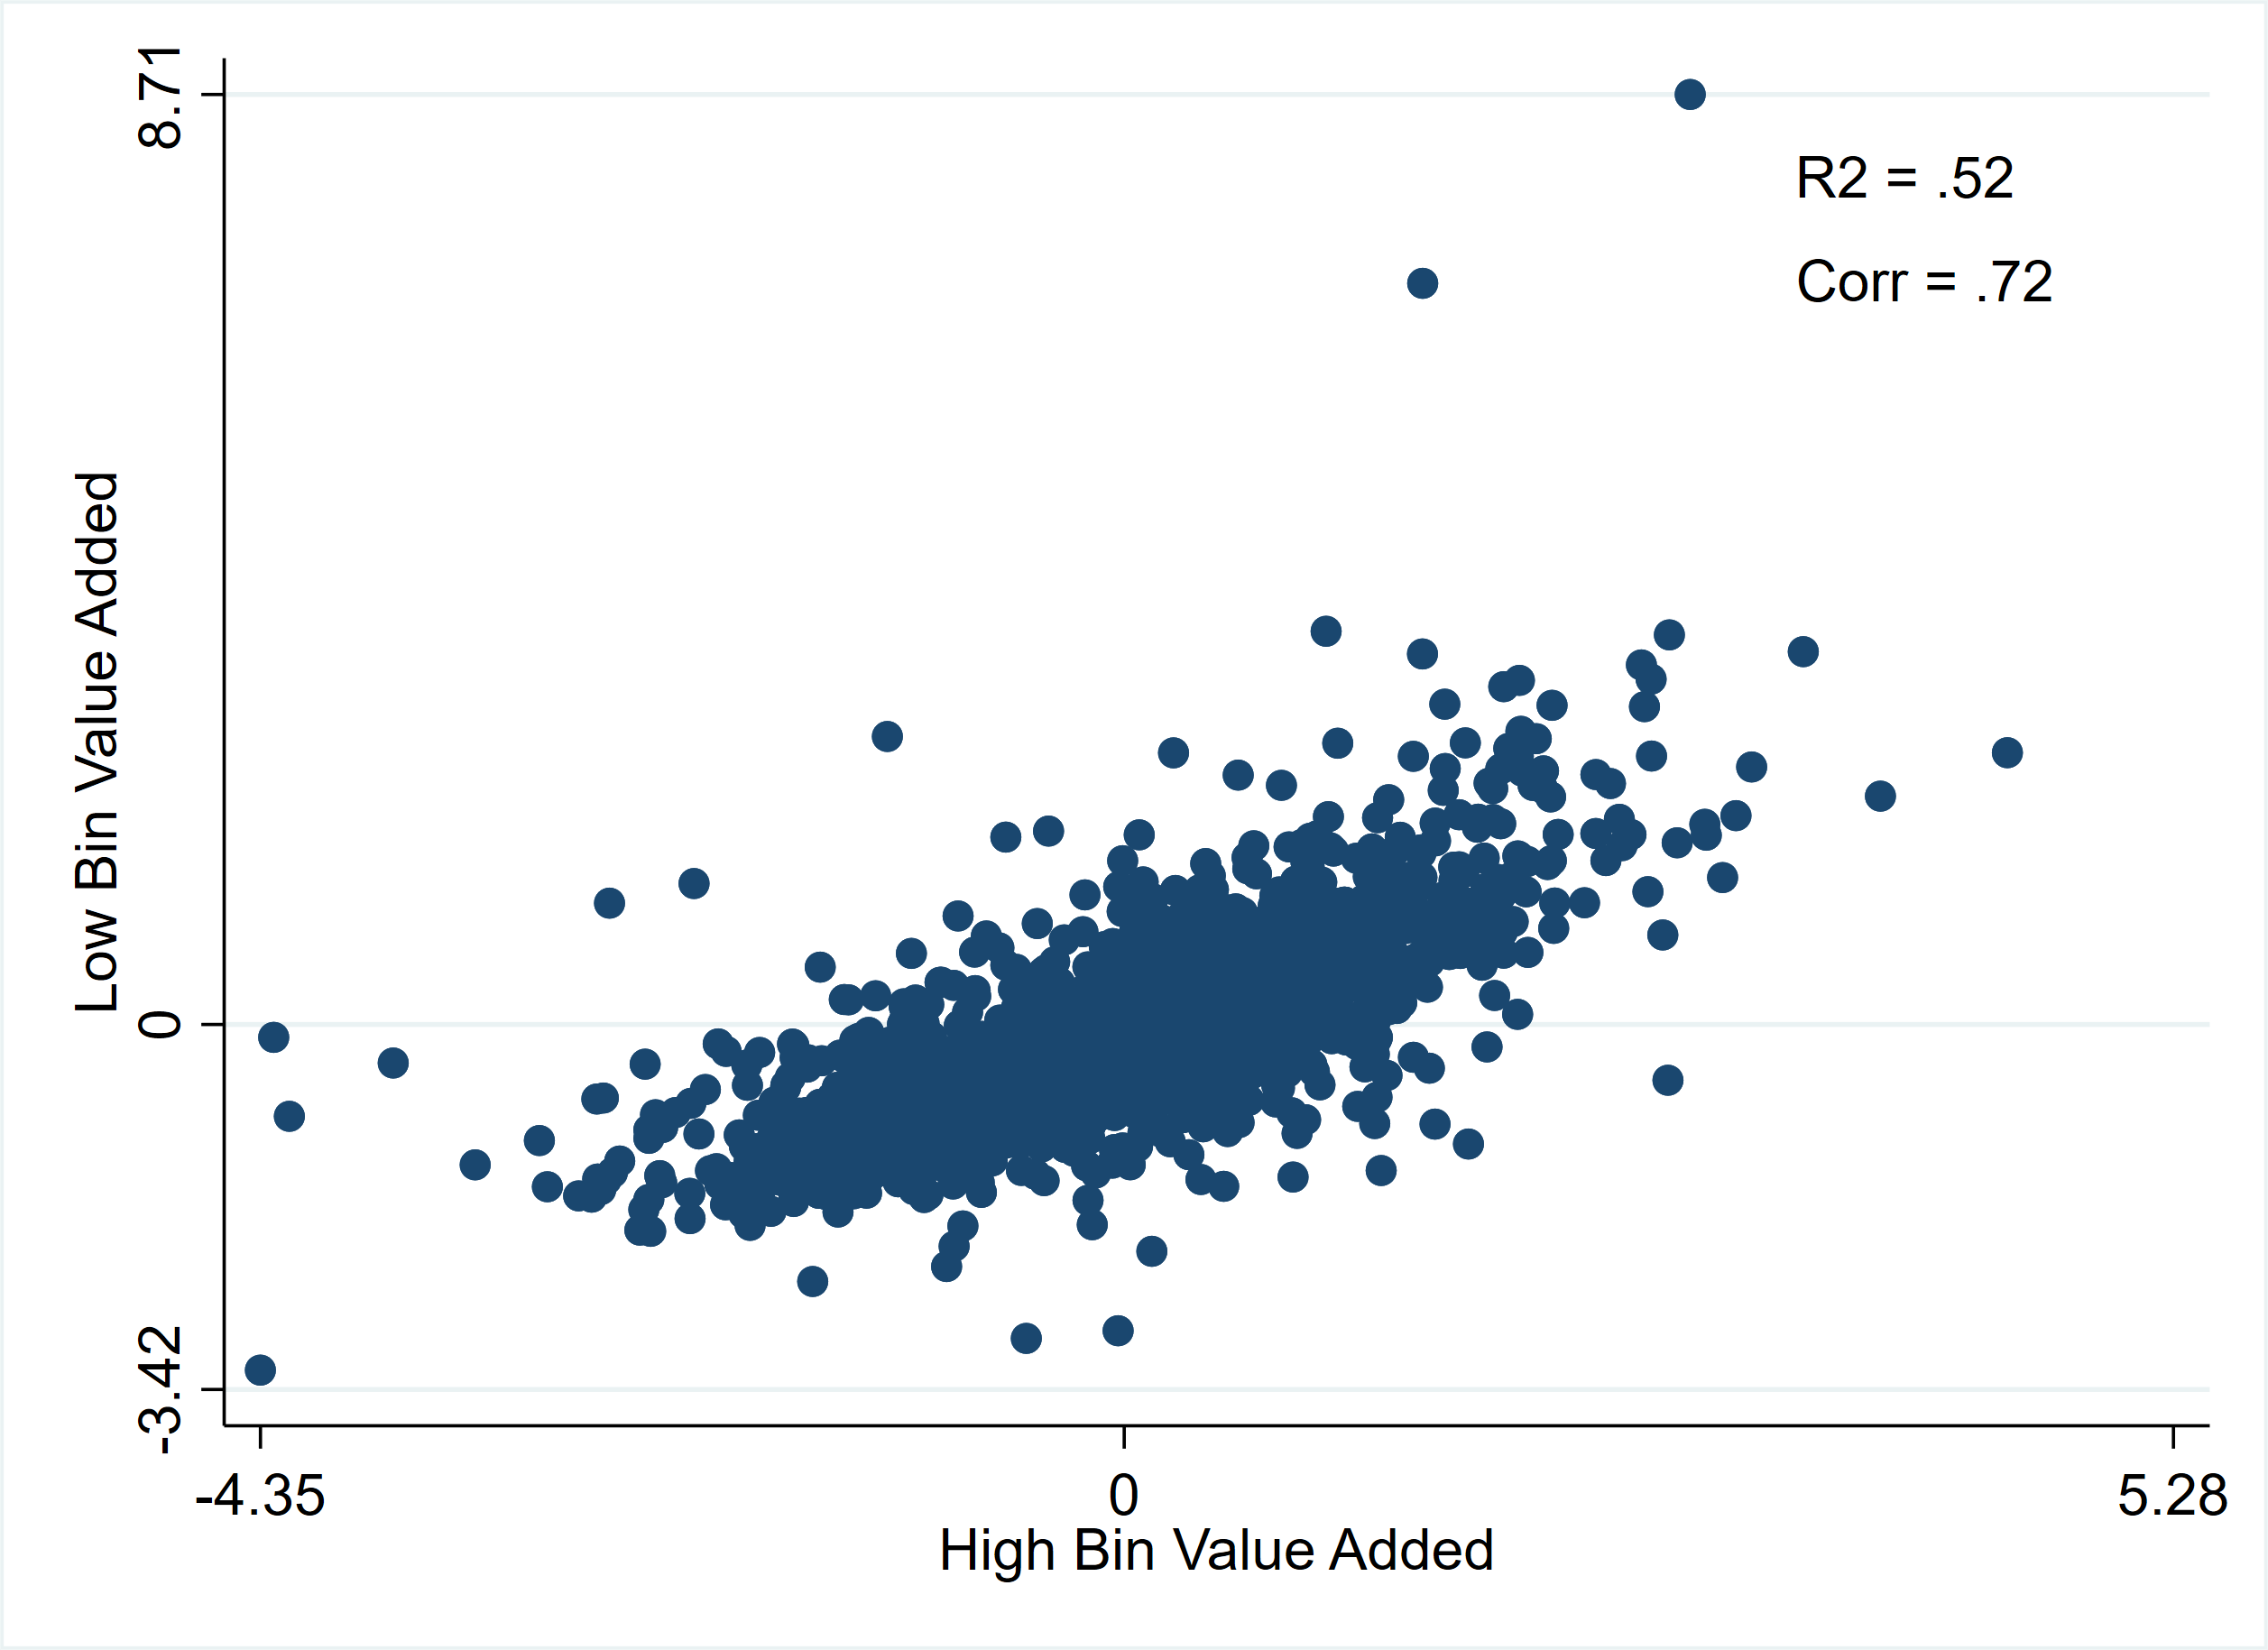
\includegraphics[width=\textwidth]{figures/Math_High_Bin_Versus_Low_Bin.png}
    \label{fig: math corr}
\end{figure}

\begin{figure}[ht]
    \centering
    \caption{Sorting by Prior Year Math Score with 2 Bins, Min 50 Students per Teacher}
    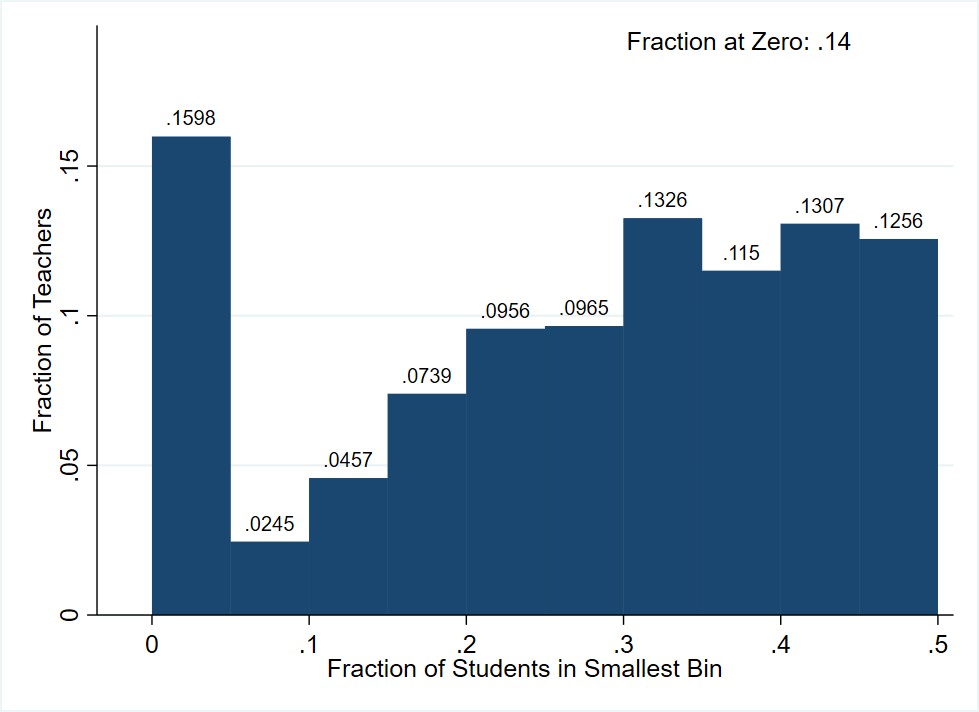
\includegraphics[width=\textwidth]{figures/ELA_Sorting_2_50.png}
    \label{fig: Math sort 2 50}
\end{figure}

\begin{figure}[ht]
    \centering
    \caption{Sorting by Prior Year Math Score with 4 Bins, Min 50 Students per Teacher}
    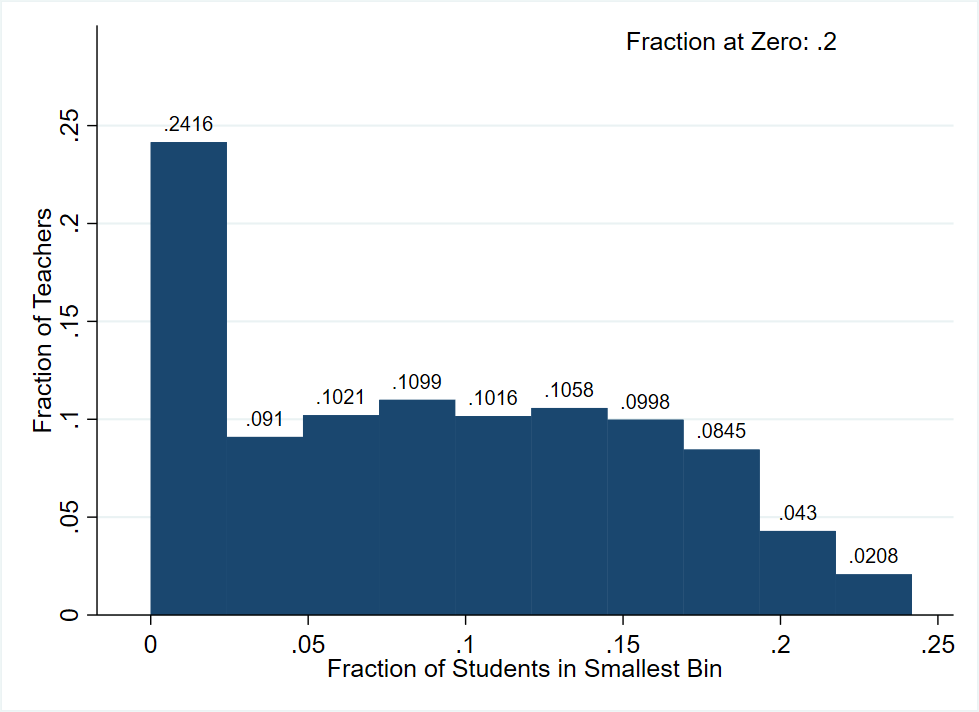
\includegraphics[width=\textwidth]{figures/ELA_Sorting_4_50.png}
    \label{fig: Math sort 4 50}
\end{figure}

\begin{figure}[ht]
    \centering
    \caption{Sorting by Prior Year Math Score with 2 Bins, Min 200 Students per Teacher}
    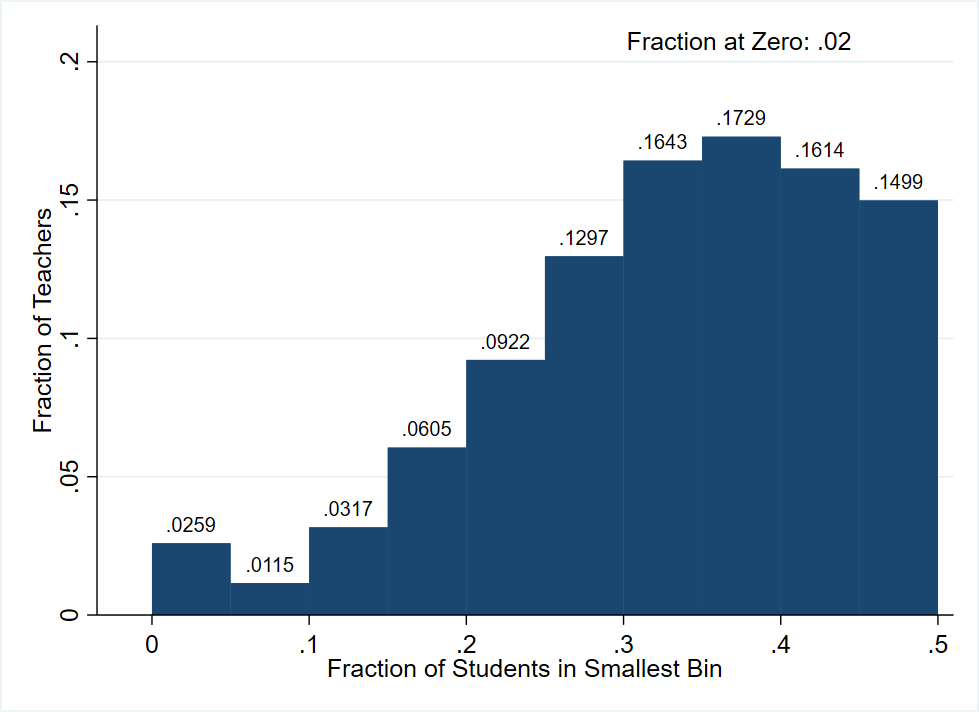
\includegraphics[width=\textwidth]{figures/ELA_Sorting_2_200.png}
    \label{fig: Math sort 2 200}
\end{figure}

\begin{figure}[ht]
    \centering
    \caption{Sorting by Prior Year Math Score with 4 Bins, Min 200 Students per Teacher}
    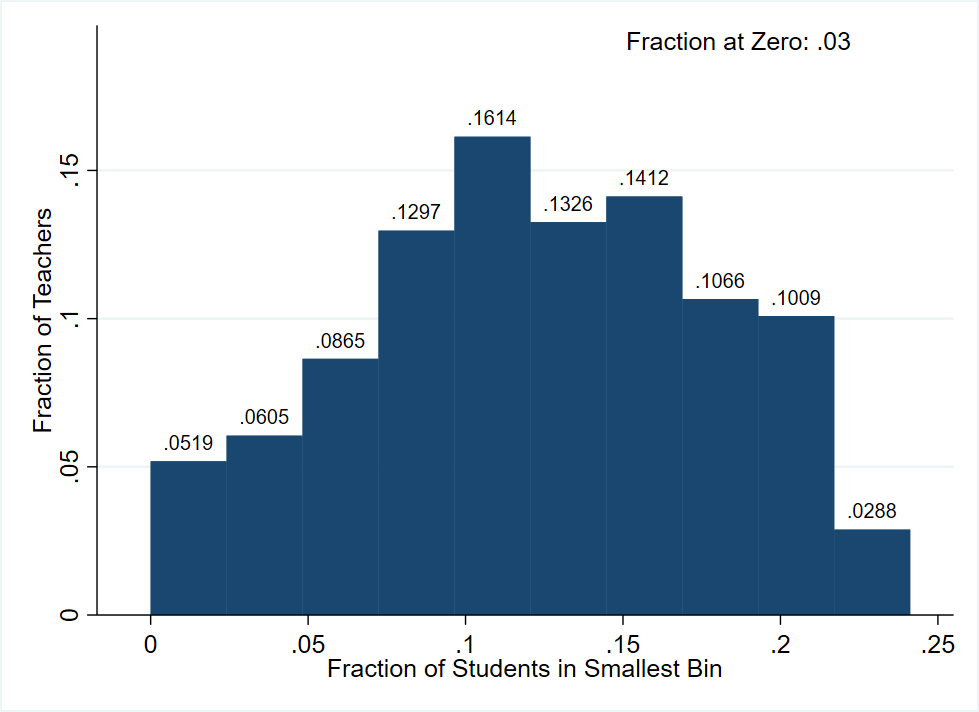
\includegraphics[width=\textwidth]{figures/ELA_Sorting_4_200.png}
    \label{fig: Math sort 4 200}
\end{figure}


\end{document}